\chapter{Beyond classical Turing patterns}\label{Chapter 1}
\section{Synopsis}
The Turing instability is a well-known mechanism for pattern formation.
Turing instabilities are defined and studied using linear stability analysis, but can also be further explored with numerical methods.
Linear stability analysis (LSA) predicts whether a pattern will occur through the dispersion relation, where the real part of eigenvalues determines the stability of the system as a function of a wavenumber parameter.
Although faster, this method provides less insights into the pattern that emerges, as it relies on the linearisation around the steady state.
On the other hand numerical methods, which are more computationally expensive, provide a detailed result of the developing pattern as the concentration of species in time and space.
Numerical results also allow us to visualize the resulting Turing pattern shape, which in 2D can consists of spots, stripes or labyrinths.

To effectively conduct a high-throughput study exploring the \#1754 synthetic Turing gene circuit, it's essential to leverage LSA.
LSA offers a much quicker alternative compared to numerical methods for understanding the patterning capabilities of the experimental circuit.
However, LSA, which relies on linearization around the steady state, sometimes fails to predict pattern formation accurately.
Understanding what information can be obtained from LSA before resorting to numerical methods, and when do LSA predictions break will enable us to efficiently gather extensive insights into both the patterning potential and the robustness of the system.

In this chapter, we first study the relationship between the analytical dispersion relation and the numerical results in Turing patterns.
This includes understanding how to predict wavelength,
convergence time and even pattern shape from the dispersion relation.
This is important to obtain information from the emergent pattern without having to solve the PDE numerically.
Then we explore how LSA might not always be a good predictor of pattern formation.
For example, how multistability can break LSA predictions and how other types of dispersion relation profiles or instabilities which are not classical Turing can generate stationary spatial patterns or other types of temporal-spatial patterns.
Finally, we explore numerically how these patterns behave when realistic biological features present in our experimental setup are introduced, such as absorbing boundaries or growth.



\section{Linear stability analysis and the dispersion relation}\label{lsa}
\subsection{Linear stability analysis for a reaction-diffusion system}


The following section describes how LSA is carried out for the steady states in a reaction-diffusion system.
The aim of this analysis is to find out if the steady state exhibits a Turing instability which is also called a diffusion-driven instability.
When it does, the system is capable of forming spatial patterns at least transiently.
As the name describes, diffusion-driven instabilities arise in these systems when a homogeneous steady state is stable to small perturbations in the absence of diffusion, and becomes unstable in the presence of diffusion~\parencite{Glendinning1994, J.DMurray2002}.
To check for Turing instabilities, the stability of the equilibrium state will be studied without and with diffusion.
The method of LSA will be explained for the two morphogen reaction-diffusion system, shown below:


\begin{subequations}
    \begin{equation}
        \pdv{A}{t}= f_{A}(A, I) + D_{A}\nabla^2 A
        \label{eq:RD general equation 1}
    \end{equation}
    \begin{equation}
        \pdv{I}{t} = f_{I}(A, I) + D_{I}\nabla^2 I
        \label{eq:RD general equation 2}
    \end{equation}
    \label{eq: RD general equations}
\end{subequations}
where $f_{A,I}$ are the non-linear production terms and $D_{A,I}$ are the diffusion constants of the two morphogens.

\subsubsection{Stability of steady state without diffusion}
To study the stability around the steady state without diffusion, only the reaction terms of Eqs.\ref{eq: RD general equations} are used:
\begin{subequations}
    \begin{equation}
        \pdv{A}{t} = f_{A}(A,I)
    \end{equation}
    \begin{equation}
        \pdv{I}{t} = f_{I}(A,I)
    \end{equation}
    \label{eq: R general equations}
\end{subequations}
There is no space dependence here as diffusion terms have been removed.
Therefore, there is only time dependence.
The steady states are defined as $A^*$ and $I^*$, which satisfy the condition:
\begin{equation}
    f_{A}(A^*,I^*)=0, \hspace{1.5cm} f_{I}(A^*,I^*)=0
\end{equation}
In this section, X is a vector with the two morphogens $X=[A,I]$.
LSA is carried by adding an infinitesimally small perturbation $\delta X$ to the steady state $X^*$, and studying if the perturbation decays (stable steady state) or grows (unstable steady state) over time.
 The perturbation needs to be almost insignificant as Taylor expansion is carried out to linearise the system around the steady state. Therefore, the morphogen concentration can be expressed as:
\begin{subequations}
    \begin{equation}
        A(t) = A^* + \delta A(t),\hspace{1.5cm} |\delta A| <<A^*
    \end{equation}
    \begin{equation}
        I(t) = I^* + \delta I(t), \hspace{1.5cm} |\delta I| <<I^*
    \end{equation}
    \label{eq: steady states}
\end{subequations}
The differential Eqs. \ref{eq: R general equations} are evaluated at steady state, using Eqs~\ref{eq: steady states}:
\begin{subequations}
    \begin{equation}
        \pdv{A}{t} = \pdv{[A^* + \delta A(t)]}{t} = f_{A}(A^* + \delta A(t), I^* + \delta I(t)) = \pdv{\delta A}{t}
    \end{equation}
    \begin{equation}
        \pdv{I}{t} = \pdv{[I^* + \delta I(t)]}{t} = f_{I}(A^* + \delta A(t), I^* + \delta I(t)) = \pdv{\delta I}{t}
    \end{equation}
    \label{eq: R equations at steady state}
\end{subequations}
As previously mentioned, the non-linear system will be linearised around the steady state using Taylor expansion.
This is done to have a simpler set of equations, that represent the system around the steady state, as seen below:
\begin{equation}
    \begin{split}
         f(A^*+\delta A, I^*+\delta I) =  f(A^*,I^*) + \pdv{f(A^*,I^*)}{A}\delta A + \pdv{f(A^*,I^*)}{I}\delta I + \dots  \\\\ + \frac{1}{n!} \pdvn{n}{f(A^*,I^*)}{A}\delta A^n + \frac{1}{n!} \pdvn{n}{f(A^*,I^*)}{I}\delta I^n
    \end{split}
\end{equation}



%\begin{split}
%    \pdv{[X(x,t)]}{x}) = \mathcal{F}^{-1}\left(\pdv{[X(k,t)]}{x}\right) = \frac{\partial}{\partial x}\left[\frac{1}{2\pi}\int_{-\infty}^{\infty} X(k,t)e^{ikx} dk\right] =  \frac{1}{2\pi}\int_{-\infty}^{\infty} X(k,t)\frac{d}{dx}e^{ikx} dk\\\\ =\frac{1}{2\pi}\int_{-\infty}^{\infty} ik X(k,t)e^{ikx} dk = ik \frac{1}{2\pi}\int_{-\infty}^{\infty} X(k,t)e^{ikx} dk = ik X(x,t)
%\end{split}




If $\delta A$ and $\delta I$ are small enough, higher order terms can be ignored as $\delta (A,I)^n$  becomes infinitesimally small.
Furthermore, it can be assumed that $f(A^*,I^*) = 0$, therefore the following expression is obtained, where $f$ corresponds to either $f_{A}$ or $f_{I}$  :
\begin{equation}
    f(A^*+\delta A, I^*+\delta I) =  \pdv{f(A^*,I^*)}{A}\delta A + \pdv{f(A^*,I^*)}{I}\delta I
\end{equation}
Finally, because $\pdv{X}{t} =  \pdv{\delta X}{t}$  at steady state (Eqs. \ref{eq: R equations at steady state}), the change in perturbation, meaning decay or growth, can be expressed as:
\begin{subequations}
    \begin{equation}
        \pdv{\delta A}{t} = \pdv{f_{A}(A^*,I^*)}{A}\delta A + \pdv{f_{A}(A^*,I^*)}{I}\delta I
    \end{equation}
    \begin{equation}
        \pdv{\delta I}{t} = \pdv{f_{I}(A^*,I^*)}{A}\delta A + \pdv{f_{I}(A^*,I^*)}{I}\delta I
    \end{equation}
    \label{eq: linearised terms around steady state}
\end{subequations}


The general solution can be expressed as an exponential, where $\sigma$ determines the growth rate of the perturbation, and whether it grows (unstable steady state) or decays (stable steady state):
\begin{subequations}
    \begin{equation}
        \delta A = A_{0}e^{\sigma t}
    \end{equation}
    \begin{equation}
        \delta I = I_{0}e^{\sigma t}
    \end{equation}
    \label{eq: exponential R}

\end{subequations}
If Eq. \ref{eq: exponential R} are introduced into Eq. \ref{eq: linearised terms around steady state}, and the solution divided by $e^{\sigma t}$ on both sides, the following is obtained:
\begin{subequations}
    \begin{equation}
        \sigma \delta A_{0} = \pdv{f_{A}(A,I)}{A} \delta A_{0} + \pdv{f_{A}(A,I)}{I}\delta I_{0}
    \end{equation}
    \begin{equation}
        \sigma \delta I_{0} = \pdv{f_{I}(A,I)}{A} \delta A_{0}+ \pdv{f_{I}(A,I)}{I}\delta I_{0}
    \end{equation}
\end{subequations}
If the Jacobian J of this system is
\begin{equation}
    J = \begin{bmatrix}
            \pdv{f_{A}}{A} &
            \pdv{f_{A}}{I}  \\
            \pdv{f_{I}}{A} &
            \pdv{f_{I}}{I}
    \end{bmatrix}
\end{equation}
This can be represented as an eigenvalue-eigenvector problem using the jacobian $J$, the eigenvalue $\sigma$ and the eigenvector  $\delta X_{0} = [\delta A_{0},\delta I_{0}]$:
\begin{equation}
    \sigma \cdot \delta X_{0} = J \cdot \delta X_{0}
\end{equation}
Finally, $\sigma$ can be obtained by solving the characteristic polynomial:
\begin{equation}
    p(\sigma) = det[J-\sigma I] = 0
\end{equation}


For a system with two variables, there are two eigenvalues $\sigma_{1}$ and $\sigma_{2}$.
The real part of $\sigma$ corresponds to the growth rate of the perturbation.
$Im(\sigma)$ corresponds to the oscillations.
If all $Re(\sigma) < 0 $, the steady state will be stable to perturbations, which means the system will go back to steady state after a small perturbation is applied.
If at least one $Re(\sigma) > 0 $, the steady state will be unstable to perturbations, and the system will go away from the equilibrium point after being slightly perturbed.
The first requirement for a Turing instability is that the system without diffusion is stable, therefore all eigenvalues must be negative.
%
%-------------------
%
%This can also be written in terms of
%
%\begin{subequations}
%    \begin{equation}
%        \pdv{\delta A}{t} = a_{11}\delta A + a_{12}\delta I
%    \end{equation}
%    \begin{equation}
%        \pdv{\delta I}{t} =  a_{21}\delta A +  a_{22}\delta I
%    \end{equation}
%\end{subequations}
%
%where
%
%\begin{subequations}
%    \begin{equation}
%        a_{11} = \pdv{f_{A}(A^*,I^*)}{A} \hspace{1.5cm} a_{12} = \pdv{f_{A}(A^*,I^*)}{I}
%    \end{equation}
%    \begin{equation}
%        a_{21} = \pdv{f_{I}(A^*,I^*)}{A} \hspace{1.5cm} a_{22} = \pdv{f_{I}(A^*,I^*)}{I}
%    \end{equation}
%
%\end{subequations}
%
%It can also be expressed in terms of the jacobian J
%
%\begin{equation}
%    J = \begin{bmatrix}
%                              \pdv{f_{A}}{A} &
%                              \pdv{f_{A}}{I}  \\
%                              \pdv{f_{I}}{A} &
%                              \pdv{f_{I}}{I}
%    \end{bmatrix}
%    = \begin{bmatrix}
%          a_{11} &
%          a_{12} \\
%          a_{21} &
%          a_{22}
%    \end{bmatrix}
%\end{equation}
%
%For a vector U
%
%
%\begin{subequations}
%    \begin{equation}
%        U = \begin{bmatrix}
%                \delta A  \\
%                \delta I
%        \end{bmatrix},   \hspace{0.5cm}  \pdv{U}{t} = J \cdot U
%    \end{equation}
%\end{subequations}
%
%
%
%
%Diagonalisation can be applied to obtain an exponential solution for the perturbations $\delta A$ and $\delta B$ in terms of the eigenvalues $\sigma_{1}$ and $\sigma_{2}$ where $c_{1}, c_{2}, c_{3}, c_{4}$ are constants
%
%\begin{subequations}
%    \begin{equation}
%    \delta A(t) = c_{1}e^{\sigma_{1}t} + c_{2}e^{\sigma_{2}t}
%    \end{equation}
%
%    \begin{equation}
%        \delta I(t) = c_{3}e^{\sigma_{1}t} + c_{4}e^{\sigma_{2}t}
%    \end{equation}
%\end{subequations}


\subsubsection{Stability of steady state with diffusion}
Once the stability of the steady state has been analysed in the absence of diffusion, the effect of diffusion on the same system will be studied.
The diffusion will be introduced through the partial derivative term $D_{X}\nabla^2 X$.




\paragraph{Definition of a function in a finite system with no-flux boundary conditions:}
A function X(x), which represents concentration of molecule X in space x, is defined in a finite-domain [0,L] with no-flux boundary conditions.
No-flux boundary conditions imply that the derivative of the function at the boundaries is zero:

\begin{equation}
    \frac{\partial X}{\partial x}\Bigg|_{x=0} = \frac{\partial X}{\partial x}\Bigg|_{x=L} = 0
\end{equation}


A general Fourier series representation of X(x) under these conditions can be:

\begin{equation}
    X(x) = \sum_{n=0}^{\infty} \left( A_n \cos\left(\frac{n \pi x}{L}\right) + B_n \sin\left(\frac{n \pi x}{L}\right) \right)
\end{equation}

However, because the derivative at the boundary is zero, the cosine series is used instead.
This is because the derivative of $\cos(0)$ or $\cos(n\pi)$ is zero.
Therefore, the Fourier cosine series used is
%TODO add cos_boundary_conditions.pdf

\begin{equation}
    X(x) = \sum_{n=0}^{\infty}  C_n \cos\left(\frac{n \pi x}{L}\right)
    \label{cosine_series}
\end{equation}

This way, if the function X(x) is expressed in terms of cosines, the derivatives of this function for x=0 and x=L are zero:
\begin{equation}
    \frac{\partial \left(cos(0)\right)}{\partial x} = 0 ; \quad \frac{\partial \left(cos(\frac{n \pi L}{L})\right)}{\partial x} = 0
    \end{equation}

\paragraph{Derivative of function in space:}
The Laplacian Operator $\nabla^2$ is applied to X(x) to represent the diffusion terms
\begin{equation}
    \nabla^2 X(x) = \frac{\partial^2}{\partial x^2} \left(\sum_{n=0}^{\infty}  C_n \cos\left(\frac{n \pi x}{L}\right) \right)  = - \sum_{n=0}^{\infty}  C_n \left(\frac{n \pi }{L}\right)^2 \cos\left(\frac{n \pi x}{L}\right)
\end{equation}

If we replace the original cosine series expressing X(x) (Eg.~\ref{cosine_series}) into this equation, we obtain
\begin{equation}
    \nabla^2 X(x) = -\left(\frac{n \pi }{L}\right)^2 X(x)
\end{equation}


\paragraph{Wavenumber definition:}
The wavenumber $k$, is the spatial frequency of the wave, measured in cycles or radians per unit distance.
In this case, the wave X(x) is expressed in cosine form.
As previously explained, to satisfy the no-flux boundary conditions, the derivative of this cosine must be zero at the boundaries $x=[0,L]$.
Therefore, $k_{n}$ must be
\begin{equation}
    k_{n}=\frac{n \pi}{L}
\end{equation}

Once $k_{n}$ is defined for our boundary conditions, the expression for the Laplacian becomes

\begin{equation}
    \nabla^2 X(x) = - k_{n}^2  X(x)
    \label{eq: simplified fourier diffusion}
\end{equation}




%
%
%\paragraph{Reduction of PDE term to ODE through Fourier transformations in infinite domain}
%The second order partial derivative term will be reduced to an ODE simpler term through Fourier transforms.
%Given infinite x-domain, the following Fourier transform definitions are used:
%\begin{subequations}
%    \begin{equation}
%        F(k) = \mathcal{F}(f(x)) = \int_{-\infty}^{\infty} f(x)e^{-ikx} dx
%    \end{equation}
%    \begin{equation}
%        f(x) = \mathcal{F}^{-1}(F(k)) = \frac{1}{2\pi}\int_{-\infty}^{\infty} F(k)e^{ikx} dk
%        \label{eq:inverse fourier}
%    \end{equation}
%\end{subequations}
%First, using the inverse Fourier transform (Eq.~\ref{eq:inverse fourier}), the first order partial derivative will be reduced to an ODE form:
%\begin{equation}
%    \begin{split}
%        \pdv{[X(x,t)]}{x}) = \mathcal{F}^{-1}\left(\pdv{[X(k,t)]}{x}\right) = \frac{\partial}{\partial x}\left[\frac{1}{2\pi}\int_{-\infty}^{\infty} X(k,t)e^{ikx} dk\right] =  \frac{1}{2\pi}\int_{-\infty}^{\infty} X(k,t)\frac{d}{dx}e^{ikx} dk\\\\ =\frac{1}{2\pi}\int_{-\infty}^{\infty} ik X(k,t)e^{ikx} dk = ik \frac{1}{2\pi}\int_{-\infty}^{\infty} X(k,t)e^{ikx} dk = ik X(x,t)
%    \end{split}
%\end{equation}
%giving $\pdv{[X(x,t)]}{x}) =  ik X(x,t)$.
%Using this expression, the inverse Fourier transform and the fact that $\pdvn{2}{X(x,t)}{x} =\left(\pdv{X(x,t)}{x}\right)^2$, the following expression is obtained:
%\begin{equation}
%    \begin{split}
%        \pdvn{2}{[X(x,t)]}{x}) = \left(\pdv{X(x,t)}{x}\right)^2 = \mathcal{F}^{-1}\left[\pdv{[ikX(k,t)]}{x}\right] = \frac{\partial}{\partial x}\left[\frac{1}{2\pi}\int_{-\infty}^{\infty} ikX(k,t)e^{ikx} dk\right] \\\\=  \frac{1}{2\pi}\int_{-\infty}^{\infty} ikX(k,t)\frac{d}{dx}e^{ikx} dk =\frac{1}{2\pi}\int_{-\infty}^{\infty} (ik)^2 X(k,t)e^{ikx} dk = -k^2 \frac{1}{2\pi}\int_{-\infty}^{\infty} X(k,t)e^{ikx} dk = -k^2 X(x,t)
%    \end{split}
%    \label{eq:fourier of our system}
%\end{equation}
%%TODO robert comment "looks complicated - you could just plug in inverse FT in second derivative, and pull integral in front of second derivative, and as integral in every term, remove"
%giving
%\begin{subequations}
%    \begin{equation}
%        \pdvn{2}{A(x,t)}{x} = -k^2\cdot A
%    \end{equation}
%    \begin{equation}
%        \pdvn{2}{I(x,t)}{x} = -k^2\cdot I
%    \end{equation}
%    \label{eq: simplified fourier diffusion}
%\end{subequations}
%This way, the second order partial derivative terms, are reduced to simpler ODE systems to be used in LSA at the expense of an extra parameter, the wavenumber.
%\paragraph{Definition of boundary conditions}
%The system is defined within some boundaries, meaning x goes from 0 to L. In this case, no molecules can leave the system, so the boundary condition applied is a zero-flux boundary condition. At the boundaries, the partial derivative is zero, defined below as Neumann Boundary conditions:
%\begin{equation}
%    \pdvn{2}{X(x=0,t)}{x}=0  \hspace{0.5cm}\And  \hspace{0.5cm}\pdvn{2}{X(x=L,t)}{x}=0
%\end{equation}
%This can be visualised as a fish tank, of length L, filled with water: water diffuses freely within the tank, but cannot diffuse outside the boundaries. In addition, the levels of water at the boundaries are not fixed. For the spatial derivatives to be zero at the boundaries, some restrictions will need to be applied. The expression from Eq.~\ref{eq:fourier of our system} will be used to apply our boundary conditions.
%\begin{equation}
%    \begin{split}
%        \pdvn{2}{[X(x,t)]}{x}) =  -k^2 \frac{1}{2\pi}\int_{0}^{L} X(k,t)e^{ikx} dk =  -k^2 \frac{1}{2\pi}\int_{0}^{L} X(k,t)(cos(kx)+isin(kx))dk\\\\
%        =\frac{-k^2}{2\pi}\left(\int_{0}^{L} X(k,t)cos(kx)dk + i\int_{0}^{L} X(k,t)sin(kx)dk\right)
%    \end{split}
%\end{equation}
%The first integral is integrated by parts to express the equation in terms of $\sin(kx)$:
%\begin{equation}
%    \begin{split}
%        \pdvn{2}{[X(x,t)]}{x}) = \frac{-k^2}{2\pi}\left(\left[\frac{sin(kx)}{k}X(k,t)\right]^L_{0} - \int_{0}^{L} \frac{sin(kx)}{k}\pdv{A(k,t)}{k}dk + i\int_{0}^{L} X(k,t)sin(kx)dk\right)
%    \end{split}
%\end{equation}
%As defined with the boundary conditions (Equation 31), the partial derivative must be 0 at $x=0$ and  $x=L$.
%Therefore, at $x=0$ and  $x=L$, $\sin(kx)=0$.
%For the two boundary conditions:
%\begin{itemize}
%    \item When $x=0$: $\sin(k\cdot0)=\sin(0)=0$.
%    \item Therefore for $x=0,\pdvn{2}{X(0,t)}{x}=0$.
%    \item When $x=L$: $\sin(k\cdot L)$ must be zero.
%    \item If $ k=\frac{n\pi}{L}$, $\sin(kL) = \sin(n\pi) = 0$.
%    Therefore, for $x=L$ , $\pdvn{2}{X(L,t)}{x}=0 \hspace{0.5cm} \forall n \in \{0, \mathbb{N}\} $
%\end{itemize}
%Following these calculations, the zero-flux boundary condition is applied if the following condition is met: $k=\frac{n\pi}{L} \hspace{0.1cm}\forall n \in \{0, \mathbb{N}\} $

\paragraph{Linear stability analysis  of steady state with diffusion effects}
Now that the PDE diffusion term has been reduced to an ODE term, and the zero-flux boundary conditions introduced, the stability of the steady state when introducing diffusion can be studied.
As shown in Eqs.~\ref{eq: simplified fourier diffusion}, the diffusion term $\nabla^2 X(x)$ can be expressed as $- k_{n}^2  X(x)$, therefore the linearised reaction-diffusion PDE equations can be written as
\begin{subequations}
    \begin{equation}
        \pdv{A}{t} = f_{A}(A^*+\delta A, I^*+\delta I)  -D_{A}k_{n}^2A
    \end{equation}
    \begin{equation}
        \pdv{I}{t} = f_I(A^*+\delta A, I^*+\delta I) -D_{I}k_{n}^2I
    \end{equation}
\end{subequations}
where $k_{n}=\frac{n\pi}{L} \hspace{0.1cm}\forall n \in \{0, \mathbb{N}\} $.

In the previous section, LSA was carried around the steady state with a perturbation $\delta X$, without including diffusion.
This resulted in the expression shown in Eq.~\ref{eq: linearised terms around steady state}, which describes the linearized reaction terms around the steady state.
By adding diffusion in the Fourier domain from Eq.~\ref{eq: simplified fourier diffusion} we obtain the following expression for the linearized reaction-diffusion system, where A and I are now a function of $k_{n}$ and $t$:

%TODO add hat?
\begin{subequations}
    \begin{equation}
        \pdv{\delta A}{t} = \pdv{f_{A}(A^*,I^*)}{A}\delta A + \pdv{f_{A}(A^*,I^*)}{I}\delta I  -D_{A}k_{n}^2\delta A
    \end{equation}
    \begin{equation}
        \pdv{\delta I}{t} =  \pdv{f_{I}(A^*,I^*)}{A}\delta A + \pdv{f_{I}(A^*,I^*)}{I}\delta I  -D_{I}k_{n}^2\delta I
    \end{equation}
    \label{eq:linearised RD}
\end{subequations}

We wish to find a general solution of the form:

\begin{subequations}
    \begin{equation}
        \delta A = A_{0}e^{\sigma t}\cdot e^{ik_{n}x}
    \end{equation}
    \begin{equation}
        \delta I = I_{0}e^{\sigma t}\cdot e^{ik_{n}x}
    \end{equation}
    \label{eq: exponential form RD}
\end{subequations}
where $X_{0}e^{\sigma t}$ represents the amplitude of the perturbations and $e^{ik_{n}x}$ represents the spatial oscillations (with $k_{n}$ as the wavenumber).
In this case, we are interested on the growth or decay of the perturbations over time.
Therefore, to observe the stability of the steady state, we will study the amplitude term ($X_{0}e^{\sigma t}$):
\begin{itemize}
    \item If $\sigma > 0$: perturbation ($\delta X$) grows making $\pdv{\delta X}{t} > 0$.
    Therefore, the steady state is unstable with diffusion.
    \item If $\sigma < 0$: perturbation ($\delta X$) decays making $\pdv{\delta X}{t} < 0$.
    Therefore, the steady state is stable with diffusion.
\end{itemize}
If Eqs.~\ref{eq: exponential form RD} are substituted into Eqs.~\ref{eq:linearised RD}, the following equations are obtained:
\begin{subequations}
    \begin{equation}
        \sigma \delta A_{0} = \pdv{f_{A}(A^*,I^*)}{A} \delta  A_{0}  + \pdv{f_{A}(A^*,I^*)}{I}\delta  I_{0} -D_{A}k_{n}^2\delta  A_{0}
    \end{equation}
    \begin{equation}
        \sigma \delta I_{0}= \pdv{f_{I}(A^*,I^*)}{A} \delta  A_{0}  + \pdv{f_{I}(A^*,I^*)}{I}\delta  I_{0}  -D_{I}k_{n}^2\delta A
    \end{equation}

\end{subequations}
If the Jacobian J of this system is
\begin{equation}
    J = \begin{bmatrix}
            \pdv{f_{A}}{A} - D_{A}k_{n}^2 &
            \pdv{f_{A}}{I}  \\
            \pdv{f_{I}}{A} &
            \pdv{f_{I}}{I} - D_{I}k_{n}^2
    \end{bmatrix}
    \label{jacobian_diffusion}
\end{equation}

these pair of equations can again be treated as an eigenvalue-eigenvector problem written in the following way:
\begin{equation}
    \sigma \cdot\delta X_{0} = J \cdot\delta X_{0}
    \label{eq: jacobian RD}
\end{equation}
where $\sigma$ can be obtained by solving the characteristic polynomial:
\begin{equation}
    p(\sigma) = det[J-\sigma I] = 0
    \label{eq: characteristic polynomial RD}
\end{equation}
In summary, to understand if perturbations around the steady state decay or grow when diffusion is introduced, Eq.~\ref{eq: characteristic polynomial RD} must be solved to obtain $\sigma$.
This characteristic polynomial is solved for a range of k's, being $k_{n}=\frac{n\pi}{L} \hspace{0.1cm}\forall n \in \{0, \mathbb{N}\} $.
The sign of $\sigma$ is studied for every $k_{n}$, resulting in the dispersion relation (Fig.~\ref{fig:turing_vs_noturing}).
If $\sigma > 0$, perturbations grow around the steady state and the system is unstable.
On the contrary, if  $\sigma < 0$, the system is stable and perturbations decay around the steady state.
More detail on LSA can be found in~\cite{J.DMurray2002} or~\cite{Glendinning1994}.

\subsubsection{Linear stability analysis implementation}
LSA is carried out with and without diffusion for all steady states of the system found using Newton-Raphson method (see Section~\ref{newton_raphson}).
The analysis is done for all $k_{n}=\frac{n\pi}{L} \hspace{0.1cm}\forall \{n \in \mathbb{N} : n \leq 5000\} $, meaning 5000 k's are sampled using linear stability analysis.
L is defined as 100mm which is based on the maximum length of our experimental system, described in Chapter~\ref{chapter3}.
LSA for a single steady state takes approximately approximately 0.5s.

\subsection{Model definition and database creation}
The system studied in this chapter consists of a 2-node Turing topology system with non-linear Hill terms.
The activator A activates itself and I, while the inhibitor I inhibits the activator A as seen in Fig.~\ref{fig:intro_to_Turing_patterns}A.
However, instead of using the linear terms used in the original Turing system Fig.~\ref{fig:intro_to_Turing_patterns}B~\parencite{Turing1952}, we use Hill terms which represent genetic regulations.
More information how these Hill terms represent gene expression regulations can be found in Section~\ref{Protein equations and gene regulation}.

\begin{subequations}
    \begin{equation}
        \pdv{[A]}{t}=b_{A}+V_{A} \cdot\frac{1}{1+\left(\frac{K{A}}{[A]}\right)^{n_{A}}}\cdot\frac{1}{1+\left(\frac{[I]}{K_{I}}\right)^{n_{I}}}-\mu_{A}\cdot[A] + D_{A}\nabla^2 [A]
%        \pdv{[A]}{t}=b_{A}+V_{A} \cdot\frac{1}{1+\left(\frac{K{A}}{[A]}\right)^{n_{A}}}\cdot\frac{1}{1+\left(\frac{[I]}{K_{I}}\right)^{n_{I}}}-\mu_{A}\cdot[A] + D_{A}(\partial_{xx} + \partial_{yy})[A]
    \end{equation}

    \begin{equation}
        \pdv{[I]}{t}=b_{I}+V_{I} \cdot\frac{1}{1+\left(\frac{K{A}}{[A]}\right)^{n_{A}}}-\mu_{I}\cdot[I] +
        D_{I}\nabla^2 [I]
%        D_{I}(\partial_{xx} + \partial_{yy})[I]
    \end{equation}

    \label{eq:turinghill}
\end{subequations}

To study this system, the parameter space is scanned using LSA and numerical methods.
The parameter space is sampled using Latin hypercube sampling (LHS) (see Fig.~\ref{fig:distributions}A) drawn from loguniform distributions (see Fig.~\ref{fig:distributions}C).
The LHS method is designed to cover the parameter space more efficiently with less samples than grid or uniform sampling~\parencite{Chrisman2014, Iman2014}.
More information on sampling and distributions can be found in Section~\ref{sampling method}, as well as the literature ranges chosen to sample from these distributions.

All results are stored in a PostgreSQL database created from scratch for this project.
This database includes a interconnected tables for model parameters, numerical parameters, analytical results, numerical solutions and pattern classification outputs.
More details on the database schema can be seen in Section~\ref{PostgreSql database}.
The creation of this PostgreSQL database was necessary to explore large parameter spaces and compare between analytical and numerical results in an efficient way.
%
%, to ensure from various parameter distributions to cover a wide variety of dynamical behaviours. Latin
%$V$ parameter is sampled using a The parameters used are x. The distribution used are x. latin hypercube. database. numerical solver.

%TODO complete param definitions
%variant0 (turinghill):
%- Vm_range = (10, 1000) loguniform
%- km_range = (0.1, 250)loguniform
%- mu_range = (0.001, 50)loguniform
%- d_B_range = (0.001, 10) loguniform
%- dA = 1 fixed
%- b = 0.01 fixed
%- n = 2 fixed

%variant11
%b_range = (10,10000) loguniform
%Vm_range = (10,10000) loguniform
%km_range = (0.1,100) loguniform
%mu_range = (1,100) loguniform
%n_range=(2,4) loguniform
%d_A = np.full((numbercombinations, 1), 0.01) fixed
%d_B= np.full((numbercombinations, 1), 10)fixed


%variant11
%b_range = (10,10000) loguniform
%Vm_range = (10,10000) loguniform
%km_range = (0.1,100) loguniform
%mu_range = (1,100) loguniform
%n_range=(2,4) loguniform
%d_A = np.full((numbercombinations, 1), 10) fixed
%d_B= np.full((numbercombinations, 1), 0.01) fixed



\subsection{Diffusion-driven instabilities in the dispersion relation}
Classical Turing patterns, also called diffusion-driven instabilities (DDI) or Turing instabilities, can be detected using LSA as described above.
In linear stability analysis, the dispersion relation is studied, which shows the dependency of the eigenvalues $\sigma$ on the wavenumber $k$ as seen in Eq.~\ref{eq: jacobian RD}.
For a Turing instability to occur, at $k=0$, $Re(\sigma)$ must be negative, meaning the system is stable without diffusion.
As diffusion is introduced and $k>0$, the system becomes unstable with $Re(\sigma)>0$.
For $k \rightarrow \inf$, the system must be stable again and the eigenvalue negative.
This is because otherwise a Turing II instability will occur where the dominant mode has infinitesimally large wavenumber meaning an infinitesimally small wavenumber.
The relationship between wavenumber $(k_{n})$ and wavelength $(\lambda)$ is
\begin{equation}
    \lambda_n = \frac{2 \pi}{k_n}
    \label{eq:wavelength_wavenumber}
\end{equation}
%TODO replace k with kn
\begin{figure}[H] % h! is a placement specifier; it tries to place the image here.
    \centering
    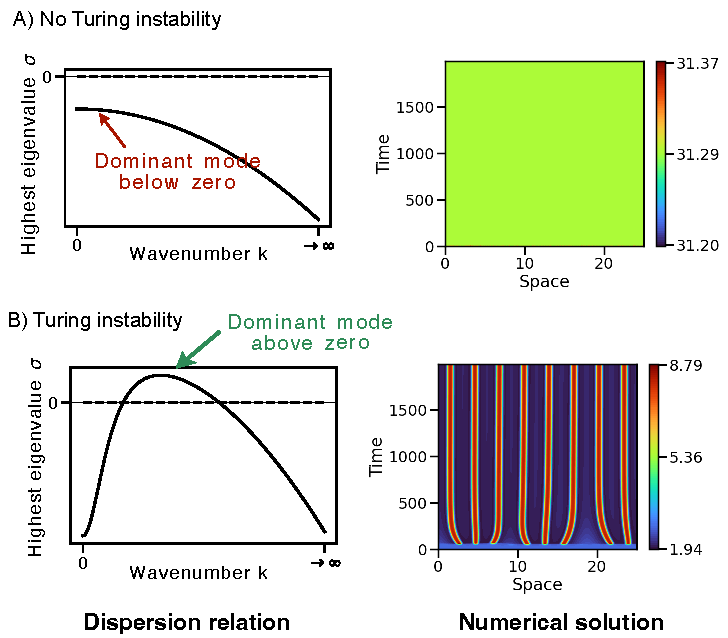
\includegraphics[width=1\textwidth]{chapters/Chapter 1/turing_vs_noturing} % The name of your image file; assumes it is in the same directory as your .tex file
    \caption{\textbf{The dispersion relation of reaction-diffusion systems.} \textbf{(A)} Dispersion relation of a system without Turing instability (left). Eigenvalues are computed for every wavenumber $k_{n}$. The dominant mode is stable, having an eigenvalue below zero. Numerical solution of system for molecule A without Turing instability (right), shows homogeneity in space (x-axis) and time (y-axis).  \textbf{(B)} Dispersion relation of a system with Turing instability (left). The dominant mode is unstable, having an eigenvalue above zero. Numerical solution of system for molecule A (right), shows a periodic in space (x-axis) which is stationary in time (y-axis). Colorbar reflects molecular species concentration.}
    \label{fig:turing_vs_noturing} % A label for referencing this figure later in the document
\end{figure}
An example of a classical Turing instability with a positive dispersion peak is shown in Fig.~\ref{fig:intro_to_Turing_patterns}B, along with the corresponding stationary spatial pattern.
Alternatively, Fig.~\ref{fig:turing_vs_noturing}A shows a spatially homogeneous solution which results from a stable system that does not exhibit a diffusion driven instability.
These 1D numerical results were produced using the \acrfull{CN} numerical scheme described in~\ref{cranknicolson}, programmed using \textit{numpy} in Python from first math principles.
The boundary conditions used here are Neumann boundary conditions where the derivative at the boundary is zero ($\pdv{U}{x}=0$) for both molecular species, A and I.

\section{Correlating linear stability analysis and numerical solutions}
\subsection{Infering wavelength and convergence time from dispersion relation}
Although LSA cannot be used to predict the final pattern, some information can be obtained from the dispersion relation.
Using the circuit defined in Eq.~\ref{eq:turinghill}, 500 parameter sets were simulated with Turing instabilities as the one seen in Fig.~\ref{fig:turing_vs_noturing}B. Subsequently, the numerical convergence time and wavelength for these patterns were measured using the algorithms described in Section~\ref{Wavelength and convergence time from numerical data}.
The predicted LSA wavelength $\lambda$ was obtained from the wavelength-wavenumber relationship (Eq.~\ref{eq:wavelength_wavenumber}) using the wavenumber $k_{n}$ which has the highest eigenvalue.

A linear relationship was found between the wavelength in the numerical pattern and the wavelength inferred from the dominant mode of the dispersion relation as seen in Fig.~\ref{fig:dispersion_to_wavelength_convergence}A. However, the slope of the regression fitted to the data is 1.46, meaning the numerical patterns obtained have a wavelength 1.46 times higher than the predicted LSA wavelength.
In terms of the convergence time, a non-linear correlation is observed between the highest eigenvalue $(\sigma)$ and the time for convergence.
Although some values do not correlate, we can overall state that systems with high eigenvalues converge faster than those with lower eigenvalues Fig.~\ref{fig:dispersion_to_wavelength_convergence}B.
However, there is a lot of noise in low eigenvalues or low convergence times.

\begin{figure}[H] % h! is a placement specifier; it tries to place the image here.
    \centering
    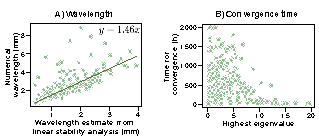
\includegraphics[width=1\textwidth]{chapters/Chapter 1/dispersion_to_wavelength_convergence} % The name of your image file; assumes it is in the same directory as your .tex file
    \caption{\textbf{Relationship between numerical wavelength or convergence, and dispersion relation features.} \textbf{(A)} Numerical wavelength with respect to wavelength predicted from linear stability analysis. Each sample which was studied analytically and numerically (light green dots). A linear regression model was applied to produce a positive correlation with slope 1.46 (dark green line). \textbf{(A)} Numerical convergence time with respect to highest eigenvalue from the dispersion relation shows a noisy decreasing function. Each sample computed numerically and analytically is a light green dot.}
    \label{fig:dispersion_to_wavelength_convergence} % A label for referencing this figure later in the document
\end{figure}

These relationships are extremely important if we wish to understand characteristics of our system such as wavelength and convergence time without simulating the system numerically.
Specially if scanning through high dimensional spaces, such methods can be extremely informative to get an insight into patterns in this space.
These relationships can be used prior to using numerical methods to choose relevant numerical parameters such as length of space and time of our simulation as well as $dx$ and $dt$.

\subsection{Dispersion to pattern shape}
To further understand the information encoded in the dispersion relation, we focused on the dispersion peak height.
The approach used consisted in optimising the dispersion peak height starting from an initial Turing pattern.
This way we can understand what happens to a specific pattern in parameter space when the dispersion peak height increases.
The optimisation is carried out using a Markov-Chain Monte Carlo combined with the Metropolis algorithm, where the optimised function is the height of the dispersion peak (i.e the highest value of the highest eigenvalue).
For more information on the optimisation algorithm, see Section~\ref{dispersion_peak_optimisation}.

For this specific optimisation work, we used a six-equation model describing the synthetic gene circuit presented in Chapter~\ref{chapter2}.
The optimisation path can be observed in Fig.~\ref{fig:dispersion_peak_optimisation}A where the dispersion peak was optimised from 0.22 to 4.36 after 50000 iterations.
This shows how the algorithm can avoid getting stuck in local maxima to go towards a global maxima.
There is no indication the algorithm is close to reaching a global maxima as the rate of improvement is still high after many iterations.
The resulting numerical patterns from the optimisation are then simulated and the convergence time measured as we did for Fig. \ref{fig:dispersion_to_wavelength_convergence}B. In Fig. \ref{fig:dispersion_peak_optimisation}B we can see a clearer correlation of how the dispersion peak height determines the convergence time which could be modelled with an exponential decay function where $x$ is dispersion peak height and$ f(x)$ is convergence time as
\begin{equation}
    f(x) = ae^{-bx} + c
\end{equation}


This optimisation was carried out for three different initial Turing parameter sets. In Fig.~\ref{fig:dispersion_peak_optimisation}C we can observe the pattern for the initial Turing pattern and the Turing pattern after optimisation (with the highest dispersion peak).
While the with lower dispersion peaks present labyrinthian type of patterns, the patterns post-optimisation present dot-like morphologies.
This suggests that a higher dispersion peak can lead to a preference for spots over labyrinths.


\begin{figure}[H] % h! is a placement specifier; it tries to place the image here.
    \centering
    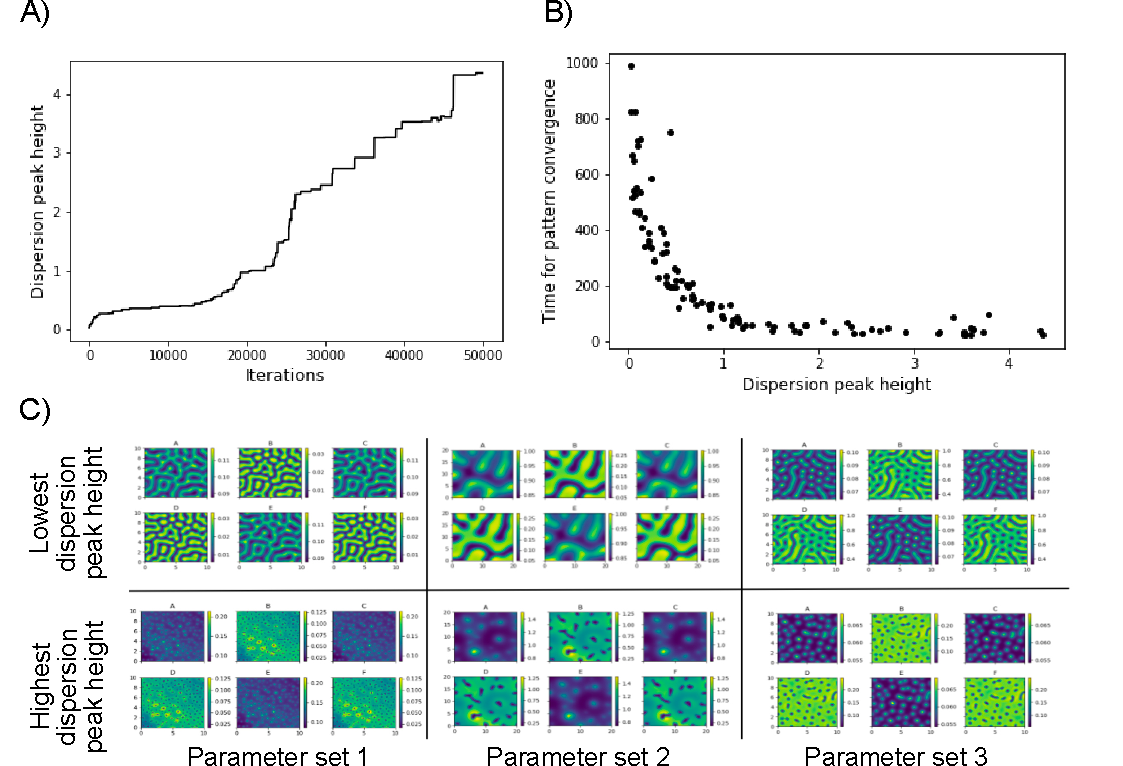
\includegraphics[width=1\textwidth]{chapters/Chapter 1/dispersion_peak_optimisation} % The name of your image file; assumes it is in the same directory as your .tex file
    \caption{\textbf{Effects of dispersion peak optimisation on convergence time and pattern shape}. \textbf{(A)} Path of the dispersion peak optimisation using the Markov-Chain Monte Carlo with Metropolis algorithm. \textbf{(B)} Numerical convergence time with respect to highest eigenvalue from the dispersion relation. Each sample computed numerically and analytically is a black dot. \textbf{(C)} Effect of dispersion peak height on pattern shape. Top figures are non optimised parameter sets (lowest dispersion peak height). The bottom figures represent parameter sets originating from the top parameter sets, that have been optimised for dispersion peak height (highest dispersion peak height). The six panels of every parameter set represent the 6 molecular species of the model.}
    \label{fig:dispersion_peak_optimisation} % A label for referencing this figure later in the document
\end{figure}



\section{Breaking linear stability analysis predictions}
Although Turing instabilities are an indicator of pattern formation, these instabilities are neither sufficient nor necessary for stationary periodic patterns to occur.
Current state-of-the-art literature analyses robustness for Turing pattern formation using LSA to determine the Turing patterning parameter space~\parencite{Scholes2019, Zheng2016, Marcon}.
With this type of analysis, you have a binary output which determines whether a parameter leads to a classical Turing instability or not as seen in Fig.~\ref{fig:lsa_numerical_confusion_literature}.
However, the assumptions depicted in this confusion matrix do not always hold true.
This is because the results from LSA give insights only into the local dynamics around a steady state.
Once the system moves away from the steady state and non-linearities are introduced, the system might behave differently and the local pattern dynamics might not be maintained.
For example, patterning instabilities that are not predicted by LSA might arise due to a subcritical bifurcation~\parencite{villar, champneys}.
This is an example of a self-organising pattern where the classical Turing instability conditions are not necessary.
.%TODO read on this

\begin{figure}[H] % h! is a placement specifier; it tries to place the image here.
    \centering
    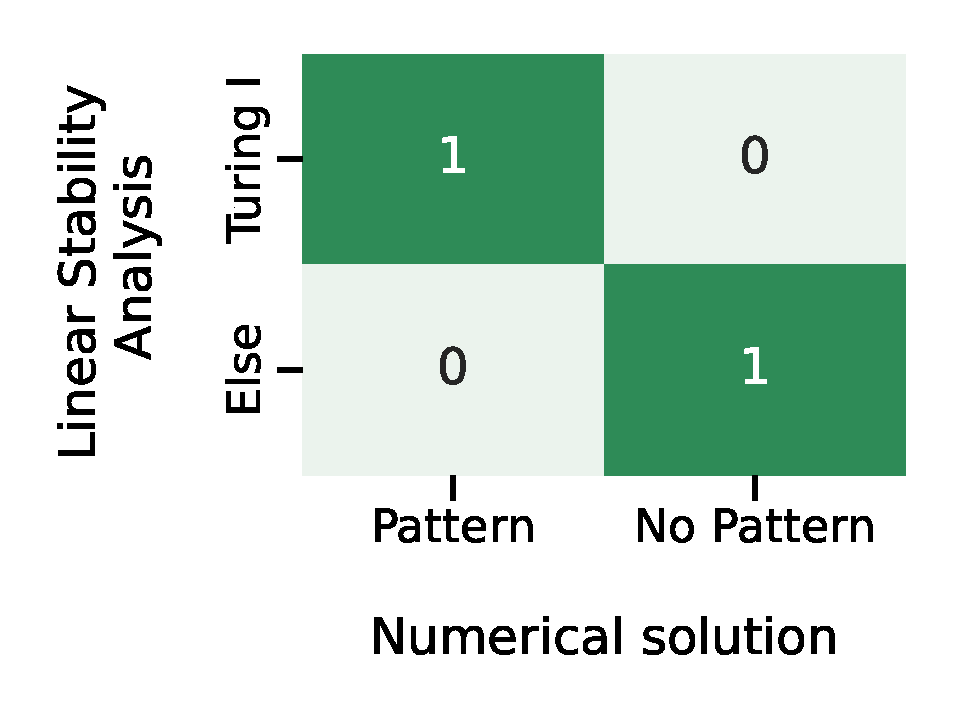
\includegraphics[width=0.6\textwidth]{chapters/Chapter 1/lsa_vs_numerical_confusion_literature} % The name of your image file; assumes it is in the same directory as your .tex file
    \caption{\textbf{Binary confusion matrix linking linear stability analysis and patterning.}}
    \label{fig:lsa_numerical_confusion_literature} % A label for referencing this figure later in the document
\end{figure}


\subsection{Multistability in Turing}
In this section, we demonstrate how linear-stability is not sufficient or necessary to predict TPs in multi-stable systems.
In particular, we study in detail the dynamical behaviour of multi-stable systems during pattern formation, which will lead to creation or breaking of the pattern.
The motivation behind this arises from the high degree of multistability exhibited by biological systems, where cell-fate decisions have to be taken within this landscape ~\parencite{huang2000shape, moris2016transition}.
Multistability is specially common in systems with non-linearities and feedback loops, as the ones in biology or in our models~\parencite{pham2020complexity, leite2009multistability}.
Using the two-node non-linear Turing topology (Eq. \ref{eq:turinghill}), multi-stable solutions were found and studied to understand how the patterning dynamics get affected when multiple steady state solutions are found.
First, LSA is carried out on a particular parameter sets to find multiple steady states of different stability (e.g.~stable, unstable, Turing I, Turing I-Hopf).
Then numerical simulations are computed where the initial condition is a random uniform distribution around a particular steady state.
Different pattern outcomes result depending on where in the phase diagram the initial condition is.
Following the classical hypothesis used in the Turing robustness literature, we would expect stable and unstable systems to not produce patterns and Turing to produce patterns.
Here, we present various examples of how this hypothesis can break under multistability conditions.

Fig.~\ref{fig:multistability1} shows a case where diffusion-driven instability conditions are not required for TP formation.
The unstable state, having a dispersion relation with a peak below zero (Fig.~\ref{fig:multistability1}C), managed to get into a TP regime as it is attracted by the Turing steady state.
It therefore produces a stationary pattern (Fig.~\ref{fig:multistability1}B), even though its dispersion relation does not predict so.
This trajectory is depicted in the phase diagram (Fig.~\ref{fig:multistability1}A) which shows the steady states along with the vector field to understand the potential trajectories of the system.

\begin{figure}[H] % h! is a placement specifier; it tries to place the image here.
    \centering
    \begin{adjustbox}{center}
        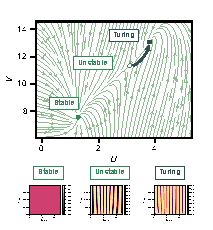
\includegraphics[width=1\textwidth]{chapters/Chapter 1/multistability1} % The name of your image file; assumes it is in the same directory as your .tex file
    \end{adjustbox}
    \caption{\textbf{Stationary Patterns in multistability.} \textbf{(A)} No diffusion phase diagram illustrating three distinct steady states where the derivative is zero: stable, unstable, and stable (Turing). These steady states are represented within a parameter space defined by two axes: concentrations of A and I. The vector field, indicated by light green arrows, shows the direction of the derivatives of the system at various points in the parameter space. A hand-drawn trajectory is also shown (dark green arrow), demonstrating how the unstable state may evolve over time into the Turing state. \textbf{(B)} Numerical solutions of the three steady states, where unstable state unexpectedly produces a Turing-like stationary pattern. \textbf{(C)} Dispersion relation showing each type of states.}
    \label{fig:multistability1} % A label for referencing this figure later in the document
\end{figure}
%TODO add stable(Turing) to text and images
%TODO clarify phase diagram is without diffusion
Then, we present a case where LSA incorrectly predicts stationary pattern formation.
Fig.~\ref{fig:multistability2} shows an ephemeral or transient pattern that occurs in the unstable and Turing regimes.
The TP initially develops in the vicinity of the Turing steady state.
As the spatial heterogeneity is amplified and settles, it gets attracted by the stable steady state leading to the disruption of the pattern.
This type of transient pattern behaviour has also been recently reported in~\cite{Krause2023}.

\begin{figure}[H] % h! is a placement specifier; it tries to place the image here.
    \centering
    \begin{adjustbox}{center}
        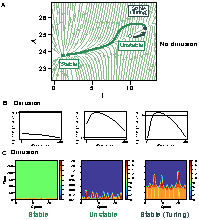
\includegraphics[width=1\textwidth]{chapters/Chapter 1/multistability2} % The name of your image file; assumes it is in the same directory as your .tex file
    \end{adjustbox}
    \caption{\textbf{Ephemeral patterns in multistability.} \textbf{(A)} No diffusion phase diagram with stable, unstable and Turing states. The hand-drawn trajectory (dark green arrow) shows unstable state evolving into stable (Turing), and stable (Turing) evolving into stable. \textbf{(B)} Numerical solutions. Unstable and Turing produce temporary periodic stationary patterns, that then dissapear and become spatially homogeneous solutions. \textbf{(C)} Dispersion relation showing each type of state.}
    \label{fig:multistability2} % A label for referencing this figure later in the document
\end{figure}

Other interesting examples can also be found, for example, where an unstable state is sourrounded by two Turing states, this unstable state will robustly lead to a Turing pattern (Fig.~\ref{fig:multistability_leftover}A).
Additionally, in some cases the unstable system settles into Turing, but the Turing system gets pulled by the stable attractor (Fig.~\ref{fig:multistability_leftover}B). Additionally, some systems it is even exhibit a transient pattern and the three solutions are homogeneous in time and space (Fig.~\ref{fig:multistability_leftover}C).
In this case, it would be worth investigating earlier timepoints with more resolution, as a pattern might appear then.
Interesting interactions similarly occur with multistability involving Turing I-Hopf solutions which will be mentioned in following sections (Fig.~\ref{fig:multistability_leftover}D).


\begin{figure}[H] % h! is a placement specifier; it tries to place the image here.
    \centering
    \begin{adjustbox}{center}
    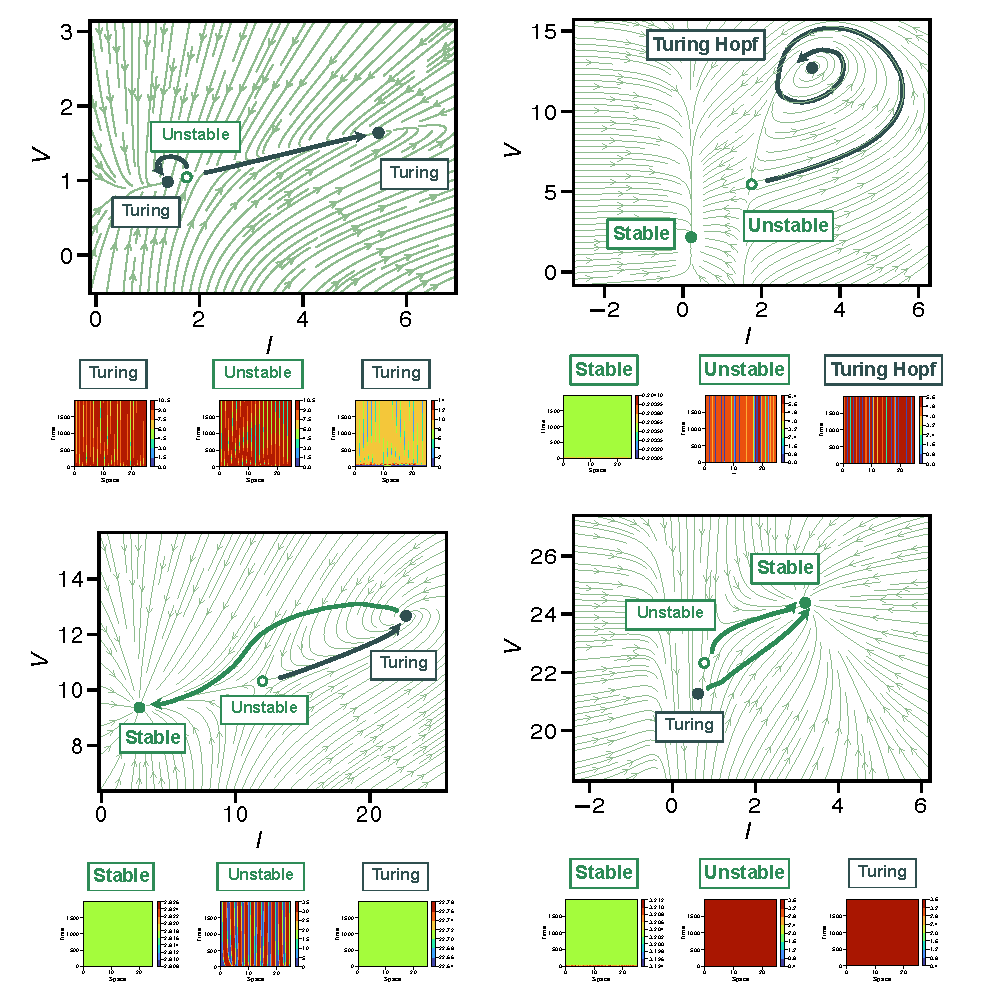
\includegraphics[width=1.2\textwidth]{chapters/Chapter 1/multistability_leftover} % The name of your image file; assumes it is in the same directory as your .tex file
    \end{adjustbox}
    \caption{\textbf{Other types of multistability dynamics.} \textbf{(A)} Unstable sourrounded by Turing robustly converges into Turing. \textbf{(B)} Unstable produces pattern, while Turing loses pattern. \textbf{(C)} Multistability disrupts all patterns. \textbf{(D)} Turing I-Hopf attracts unstable and generates pattern}
    \label{fig:multistability_leftover} % A label for referencing this figure later in the document
\end{figure}

%TODO corrected up to here

\subsection{Analytical to numerical: Other types of dispersion relations, and other types of patterns} \label{nogrowth}
Multi-stable systems are not the only case where the classical Turing instability fails to predict pattern formation.
Other types of dispersion relations beyond classical Turing instabilities can produce stationary patterns and non-stationary regular patterns that might be of interest in developmental biology.
The aim of this section is to document what type of dispersion relations in mono-stable systems can be linked to what type of patterns, to gain insights into predicting pattern formation from linear stability analysis.
We will first present a classification for the different types of dispersion relations.
Subsequently, we will show the classification for the different types of pattern outcomes, where the system is a non-growing domain with reflective boundary conditions (Neumann, where derivative is zero at the boundary).
Finally, we will reconstruct the 2x2 confusion matrix (Fig.~\ref{fig:lsa_numerical_confusion_literature}) currently used as an assumption in the literature, to show a more complete view on how to interpret dispersion relations.
The new confusion matrix will show more types of dispersion relation and more pattern outcomes leading to a 5x4 confusion matrix.

First, we classify the different dispersion relations obtained from LSA into 5 types:
\begin{itemize}
    \item Stable dispersion relations (Fig~\ref{fig:dispersions}A) have all eigenvalues $\sigma$ below zero for any wavenumber $k$.
    \item Unstable dispersion relations (Fig~\ref{fig:dispersions}B) have a positive eigenvalue at $k=0$ which eventually drops below zero as diffusion is introduced (i.e. $k>0$).
    \item Hopf-type dispersion relations, as with any unstable dispersion relation, shows an instability without diffusion ($\sigma>0$ for $k=0$) which eventually drops below zero for positive wavenumbers.
However, in the case of the Hopf-type dispersion relation, when the eigenvalues cross the zero line, there is a pair of complex conjugate eigenvalues (Fig~\ref{fig:dispersions}C).
A Hopf-like dispersion relation is different to a Hopf bifurcation: a bifurcation displays a shift in stability as a model parameter changes, while the Hopf-like dispersion is a change in stability as a function of the wavenumber $k$.
%In this case, the bifurcation parameter would be $k$, making the system go from unstable to stable by changing this parameter.
\item Turing I dispersion relations, as previously mentioned, are stable without diffusion and have an instability for a positive wavenumber and finally stable again for very large wavenumbers (Fig~\ref{fig:dispersions}D).
    \item Turing I-Hopf dispersion relations, are a combination of Turing I and Hopf-type dispersion relations.
As the Hopf-type dispersion, they are unstable without diffusion.
Then, as $k$ is increase, the system becomes stable with a pair of complex conjugates as the eigenvalues cross the zero line.
Finally, a Turing I type behaviour arises getting a peak above zero and decaying again for large wavenumbers (Fig~\ref{fig:dispersions}E).
\end{itemize}
Other types of dispersion relation exist which are not displayed here such as Turing II, where the eigenvalues do not become stable again for very large wavenumbers.
Therefore, this system displays an instability at very large wavenumbers which result in infinitesimally small wavelength patterns.
These are considered to produce homogeneous solutions, except in the case of space discretization where they can produce small wavelength patterns~\parencite{Wang2022}.
However, Turing II solutions are not possible in systems such as this one where all nodes are diffusing.
This is because for $k \rightarrow \inf$, all eigenvalues $\sigma$ must be negative (see Eq.~\ref{jacobian_diffusion}).
%TODO . They also identify examples of non-stationary spatial patterns, when the eigenvalue corresponding to a critical wave number has non-zero imaginary part.Deutsch, A., Dormann, S., et al., 2005. Cellular automaton modeling of biological pattern formation. Springer.

%TODO look at pitchfork and transcritical

\begin{figure}[H] % h! is a placement specifier; it tries to place the image here.
    \centering
    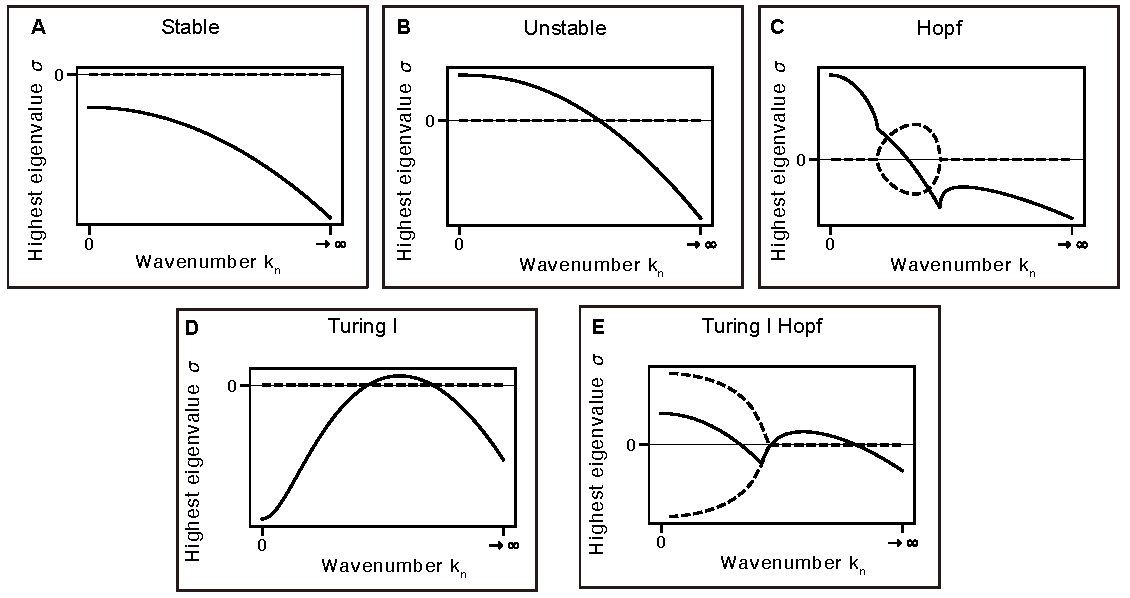
\includegraphics[width=1\textwidth]{chapters/Chapter 1/dispersions} % The name of your image file; assumes it is in the same directory as your .tex file
    \caption{\textbf{Different types of dispersion relation.} Dispersion relation shows the eigenvalue as a function of wavenumber. Continous line represents real part, while dotted line represents imaginary part. \textbf{(A) Stable:} all eigenvalues are below zero. \textbf{(B) Unstable:} eigenvalues at $k_{n}$=0 are positive meaning the system is unstable without diffusion. \textbf{(C) Hopf:}~unstable type, with hopf bifurcation for parameter wavenumber $k_{n}$. For a certain $k_{n}$, system flips from unstable to stable, crossing the zero eigenvalue line. At the crossing, there is a pair of complex conjugate eigenvalues. \textbf{(D) Turing I:} the dispersion shows a diffusion driven instability. At $k_{n}$=0, the system is stable has negative eigenvalues. As diffusion is introduced, $k_{n}$>0, the system becomes unstable and stable again for high $k$ values. \textbf{(E) Turing I-Hopf:} a combination of Turing I and Hopf, meaning the system starts as a Hopf with a positive eigenvalue at $k_{n}$=0, then the system transitions to stable with a pair of complex conjugates. Finally, there is a dispersion peak characteristic of Turing that drops for high values of $k$.}
    \label{fig:dispersions} % A label for referencing this figure later in the document
\end{figure}

As with the classification of the dispersion relations, we develop a method to classify the patterns produced numerically into homogeneous, temporal oscillator, non-stationary pattern and stationary pattern.
By classifying both LSA and numerical outputs, we can generate a new confusion matrix with information about other types of dispersion relations and other types of spatio-temporal patterns.

We use a decision tree for the classification where the two layers are spatial homogeneity and convergence in time, as seen in Fig.~\ref{fig:no growth classification}.
This decision tree leads to the 4 types of patterns mentioned.
A pattern will be considered spatially homogeneous if the final snapshot $U$ for any of the two molecular species fulfills the following condition
\begin{equation}
    \frac{max(U) - min(U)}{max(U)} \leq 0.01
\end{equation}
A pattern will be considered converged if the last 30 timepoints for any of the two molecular species fulfills the following condition
\begin{equation}
    \frac{max(U[-30:]) - min(U[-30:])}{max(U[-30:])} \leq 0.05
\end{equation}
The thresholds chosen were fine-tuned by testing them on the numerical patterns to obtain the best classification results.
Using this two characteristics, spatial homogeneity and convergence, we can obtain 4 classes of patterns as seen in Fig.~\ref{fig:no growth classification}:
\begin{itemize}
    \item Homogeneous patterns are homogeneous in space and converge in time.
    \item Temporal oscillators, also called limit cycles, are homogeneous in space but do not converge, as they oscillate in time.
    \item Non-stationary patterns are not homogeneous in space and do not converge in time.
    \item Finally, Stationary patterns are not homogeneous in space but converge in time.
\end{itemize}

\begin{figure}[H] % h! is a placement specifier; it tries to place the image here.
    \centering
    \begin{adjustbox}{center}
    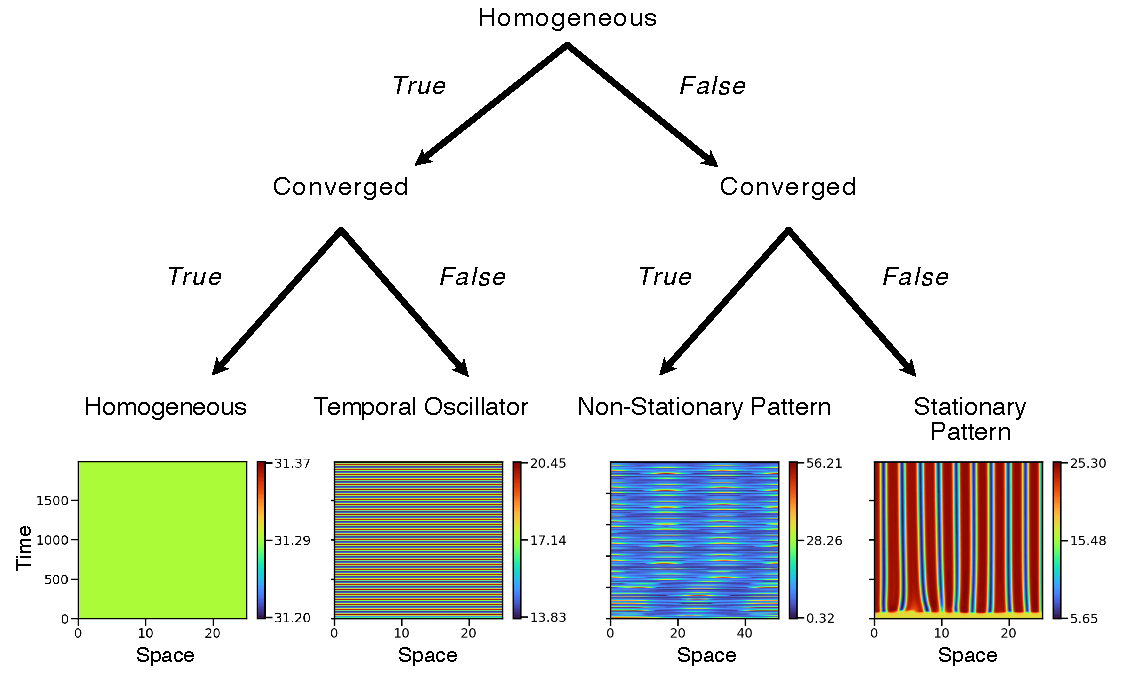
\includegraphics[width=1\textwidth]{chapters/Chapter 1/no growth classification} % The name of your image file; assumes it is in the same directory as your .tex file
    \end{adjustbox}
    \caption{\textbf{Decision tree for pattern classification in non-growing domains with reflective boundaries}. Decision tree is based on two layers: spatial homogeneity and convergence. The numerical solutions for the four different pattern outcomes including homogeneous, temporal oscillator, non-stationary pattern and stationary pattern are shown below.}
    \label{fig:no growth classification} % A label for referencing this figure later in the document
\end{figure}


High-throughput studies like~\cite{Scholes2019, Zheng2016, Marcon} only consider Turing I as patterning and the rest is discarded.
Here, we explore beyond Turing I and stationary patterns to give a more complete view of the relationship between linear stability and spatio-temporal patterns.
9,087 parameter sets are analysed from the non-linear Turing model (Eqs. \ref{eq:turinghill}) to obtain dispersion relations and numerical patterns.
Because systems such as Turing and Turing I-Hopf are undersampled in the parameter space, the dataset is enriched with them to ensure we capture enough distinct dynamical behaviors.
Multi-stable systems are not included in this analysis to understand the direct relationships between the dispersion relation and numerics.
The two types of classifications described above are applied, and a new 5x4 confusion matrix is generated (Fig.~\ref{fig:lsa_numerical_confusion}).

\begin{figure}[H] % h! is a placement specifier; it tries to place the image here.
    \centering
    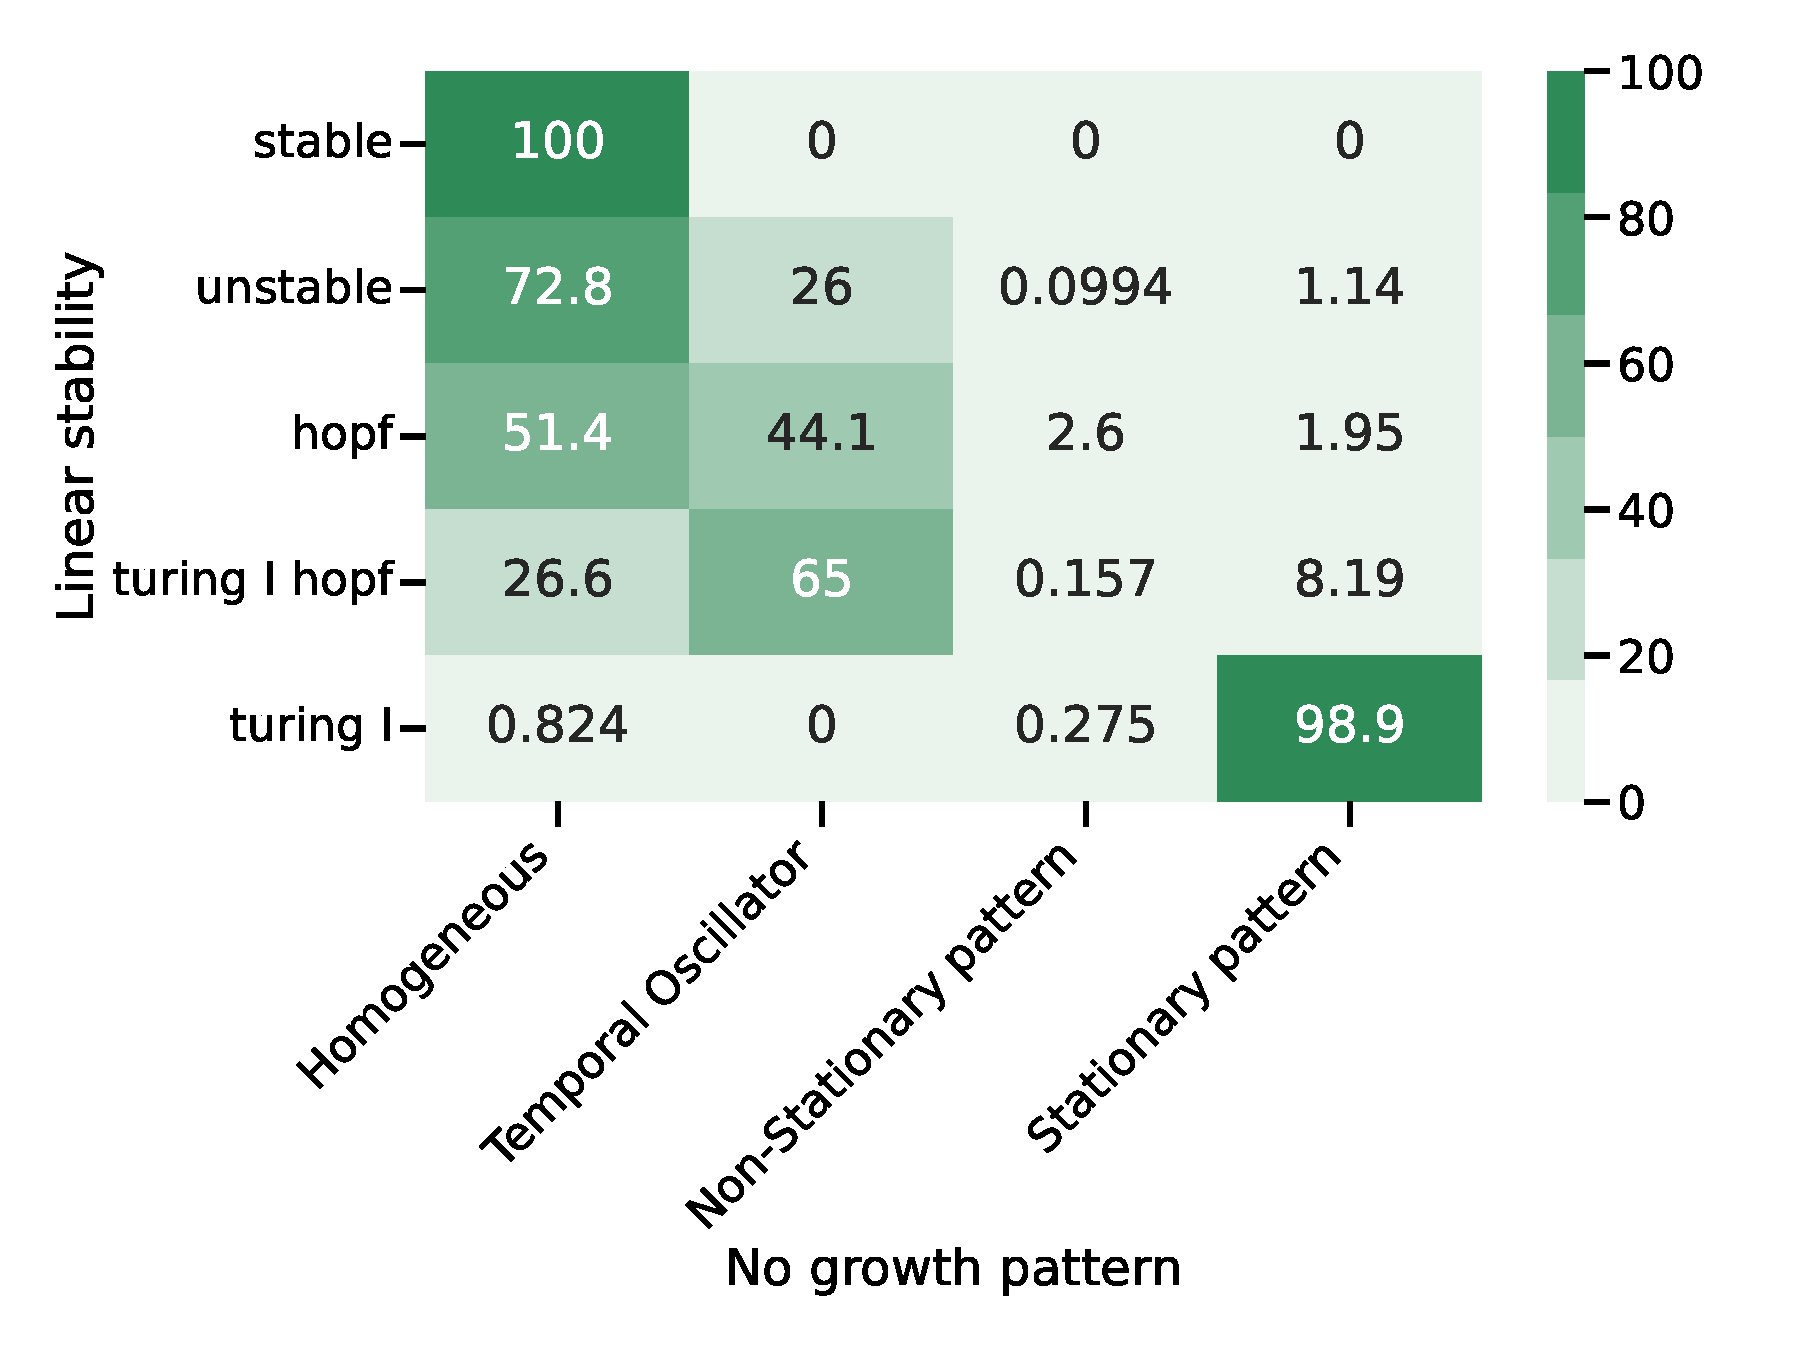
\includegraphics[width=1\textwidth]{chapters/Chapter 1/lsa_vs_numerical_confusion_variant0-11-12} % The name of your image file; assumes it is in the same directory as your .tex file
    \caption{\textbf{Confusion matrix linking LSA output (rows) and numerical pattern outcome (columns).} Numbers show the percentage of solutions across the LSA output rows.}
    \label{fig:lsa_numerical_confusion} % A label for referencing this figure later in the document
\end{figure}

It is worth pointing out some interesting examples obtained from this confusion matrix.
For example, Turing I-Hopf seems to lead to stationary patterns often (see Fig.~\ref{fig:interesting_cases_nogrowth}A), meaning they would definitely need to be included in high-throughput robustness studies.
Some unstable dispersion relations lead to both stationary (see Fig.~\ref{fig:interesting_cases_nogrowth}B) and non-stationary patterns.
Additionally, Hopf solutions also display interesting non-stationary patterns (see Fig.~\ref{fig:interesting_cases_nogrowth}C).
Unfortunately, some Hopf solutions are misclassified as Stationary patterns (see Fig.~\ref{fig:interesting_cases_nogrowth}D) due to an inadequate threshold of the convergence classification.
In this specific case, a higher window than 30 should be taken when considering convergence and a higher threshold for homogeneity.
It is important to understand that this is an initial exploratory analysis where misclassification might occur.
This is because of the difficulty of setting common thresholds for a wide variety of numerical solutions with different wavelengths, time-scales and dynamic ranges.

\begin{figure}[H] % h! is a placement specifier; it tries to place the image here.
    \centering
    \begin{adjustbox}{center}
        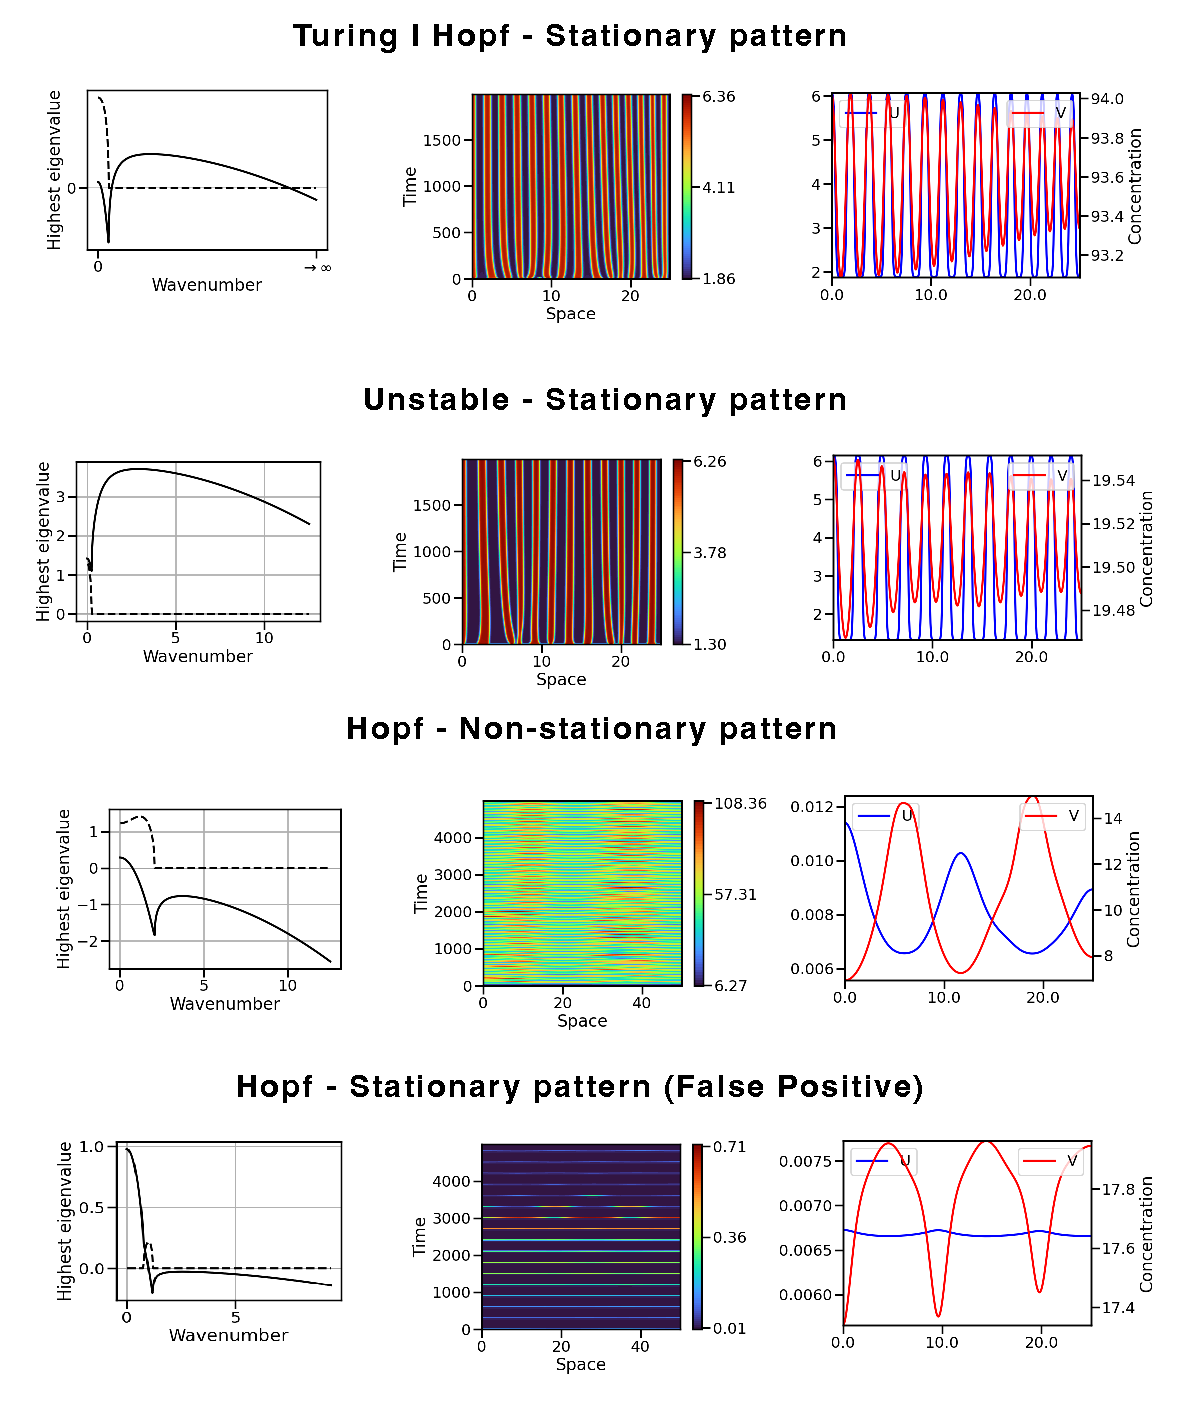
\includegraphics[width=1\textwidth]{chapters/Chapter 1/interesting_cases_nogrowth} % The name of your image file; assumes it is in the same directory as your .tex file
    \end{adjustbox}
    \caption{\textbf{Examples of numerical solutions and their respective dispersion relations.} Dispersion relation produced with LSA (left), numerical-time series (center) and final time numerical snapshot (right) produced with Crank-Nicolson. \textbf{(A)} Turing I-Hopf solution produces stationary periodic patterns. \textbf{(B)} Unstable solution produces stationary periodic patterns. \textbf{(C)} Hopf solution produces non-stationary regular patterns. \textbf{(C)} Hopf solution produces Temporal Oscillator which is misclassified as a Stationary pattern.}
    \label{fig:interesting_cases_nogrowth} % A label for referencing this figure later in the document
\end{figure}
%TODO comment mark: methods?
\section{Introducing biological features: Absorbing boundaries and growth}
As seen in the previous section, both multistability effects and numerical solutions can break the hypothesis that only classical Turing I systems can produce stationary periodic patterns.
Here, we look deeper into how other aspects linking the theory closer to the biological reality can also break this hypothesis.
In particular, we will look at how adding an absorbing boundary condition and growth to a reaction-diffusion system might induce or break patterning.
This particular direction was inspired in experiments described in the next sections where growing bacterial colonies in agar are used as a platform to engineer Turing patterns using synthetic gene circuits.

The absorbing boundaries are introduced by using a Dirilichet boundary condition where the concentration at the boundary is zero $u=0$, as opposed to the previously used Neumann boundaries where the derivative at the boundary is zero.
This particular boundary is chosen as the boundary of the colony acts as an absorbing boundary due to the lack of morphogen production in the agar.
More details on the encoding of boundaries in Crank Nicolson can be found in Fig.~\ref{fig:boundaries} or Section~\ref{methods_boundary_conditions_CN}.

Growth is introduced as apical isotropic linear growth, where cells are added to both boundaries with a linear growth rate.
More information on the different types of growth can be found in Fig.~\ref{fig:growth}.
This type of growth is inspired in linearly growing bacterial colonies where division occurs mainly in the edges.
However, in this case, solutions are in 1D to speed up computation and simplify results.
Growth of the tissue is encoded in a 1D binary vector, where cells are denoted as 1 and empty space as 0.
The number of 1's grows linearly, which represents the tissue expanding.
This vector is used as a mask, where 1's determine the computation of reaction-diffusion terms and 0's determine only the computation of diffusion.
Therefore, while reaction-diffusion occurs in the tissue; only diffusion occurs in the empty regions.
Fig.~\ref{fig:growing_pattern} shows a Turing pattern being simulated in this type of growing domain with isotropic edge growth and absorbing boundary conditions.

\begin{figure}[H] % h! is a placement specifier; it tries to place the image here.
    \centering
    \begin{adjustbox}{center}
        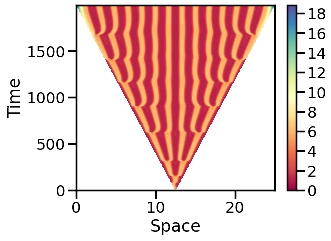
\includegraphics[width=0.5\textwidth]{chapters/Chapter 1/growing_pattern} % The name of your image file; assumes it is in the same directory as your .tex file
    \end{adjustbox}
    \caption{\textbf{Turing pattern in linearly growing domain with absorbing boundary conditions.} Time-series where X axis denotes space while Y axis denotes time. The colobar indicates the concentration of species A. Peak doubling occurs at the edges of the growing system.}
    \label{fig:growing_pattern} % A label for referencing this figure later in the document
\end{figure}

As with the non-growing reflective boundary condition patterns in the previous section (see Fig.~\ref{fig:no growth classification}), we want to classify the numerical output to quantify the different types of patterns obtained, and the transitions as absorbing boundaries and growth are introduced.
However, due to the absorbing boundary conditions and growth, patterns are rarely spatially homogeneous or converged, which makes the previous classification method unsuitable.
The new classification system is developed based on the number of peaks.
Peaks are detected using the Python $find\_peaks$ algorithm with parameter $prominence=0.05$.
Again, the thresholds for the peak finding algorithm need to be fine-tuned and depending on the numerical outcome, misclassification might occur.


\begin{figure}[H] % h! is a placement specifier; it tries to place the image here.
    \centering
    \begin{adjustbox}{center}
        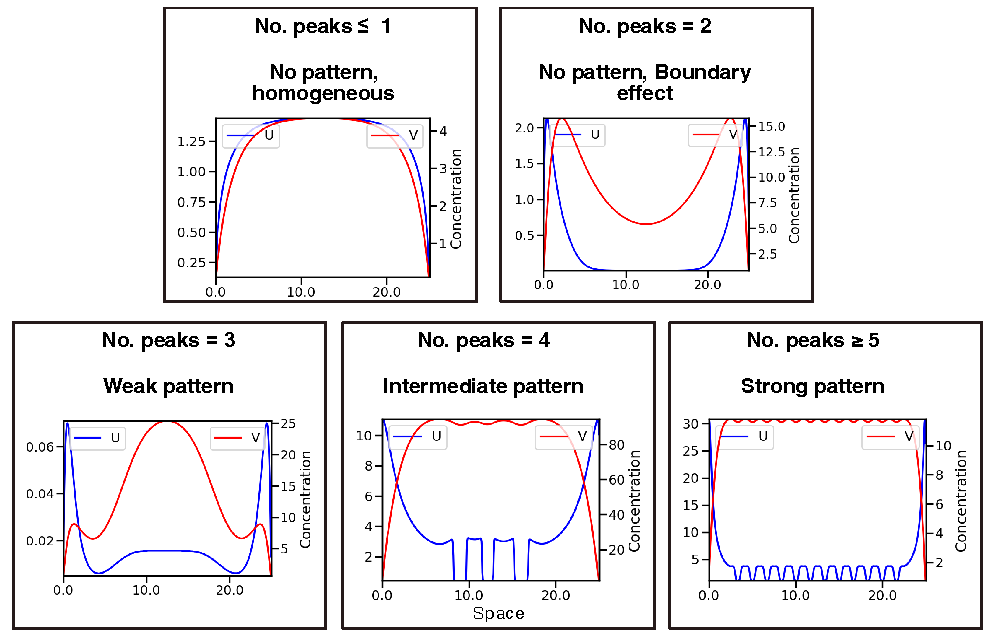
\includegraphics[width=1\textwidth]{chapters/Chapter 1/peaks_classification} % The name of your image file; assumes it is in the same directory as your .tex file
    \end{adjustbox}
    \caption{\textbf{Classification based on peaks for solutions with absorbing boundary conditions and growth.} Different numerical solutions in non-growing domains with absorbing boundary conditions classified on the basis of number of peaks. The solutions are a snapshot in time showing the concentration of A and I (shown as U and V here) in the left and right Y axis respectively. X axis designates space in mm.}
    \label{fig:peaks_classification} % A label for referencing this figure later in the document
\end{figure}
%TODO marks comment: too brief. refer to methods
The peak classification shown in Fig.~\ref{fig:peaks_classification}, retrieves information on whether there is a pattern at all and whether this pattern is only a pattern at the boundary or is a periodic pattern that would scale up with tissue length as Turing patterns do.
The 5 different types of patterns are:
\begin{itemize}
    \item Patterns with one peak will be considered homogeneous as they result from the morphogens being reduced at the boundary due to absorption (Fig.~\ref{fig:peaks_classification} no pattern, homogeneous).
    \item Patterns with two peaks are also considered not to be patterned states as the two peaks might arise at the boundary for one of the diffusors due to the depletion of the other (Fig.~\ref{fig:peaks_classification} no pattern, boundary effect).
    \item Patterns with three peaks start displaying a pattern more similar to Turing repeats, although we cannot prove the number of peaks would scale with tissue length as Turing patterns do (Fig.~\ref{fig:peaks_classification} weak pattern).
    \item Patterns with four peaks could still be purely a boundary effect, but is less likely as the number of repeats points towards tissue scaling being possible (Fig.~\ref{fig:peaks_classification} intermediate pattern).
    \item Finally, patterns with five peaks and above can be considered strong patterns and would be most similar to classical Turing patterns in non-growing no-flux boundary domains (Fig.~\ref{fig:peaks_classification} strong pattern).
\end{itemize}
Using this classification method, 9,087 parameter sets where simulated and classified with absorbing boundary conditions and growth.
Again, all these parameter sets have only a single steady state to ensure patterning effects are due to boundaries and growth and not due to multistability.


\subsection{Reflecting boundaries to absorbing boundaries}
When absorbing boundaries are added, periodic patterns might get created, disrupted or remain the same.
The confusion matrix in Fig~\ref{fig:nogrowth_openboundary_confusion_variant0} shows this transition by comparing the classification output of reflecting boundaries versus absorbing boundaries.
As previously explained, the classification in Section~\ref{nogrowth} could not be used for absorbing boundary conditions as these prevent the pattern from being completely homogeneous or stationary.
Therefore, two types of classifications have to be compared for each type of boundary.
Although the classification outputs cannot be directly compared, this confusion matrix is useful to identify interesting cases:
If absorbing boundary conditions had no effect, we would expect homogeneous and temporal oscillator categories in the y axis to become no pattern, homogeneous or boundary effect.
Additionally, we would expect stationary patterns to become strong patterns.
This is commonly the case as seen by the dark-green squares of Fig.~\ref{fig:nogrowth_openboundary_confusion_variant0}, which shows boundaries do not often affect the pattern.
However, some exceptions are present which are further studied in Fig.~\ref{fig:interesting_cases_openboundary}.

\begin{figure}[H] % h! is a placement specifier; it tries to place the image here.
    \centering
    \begin{adjustbox}{center}
        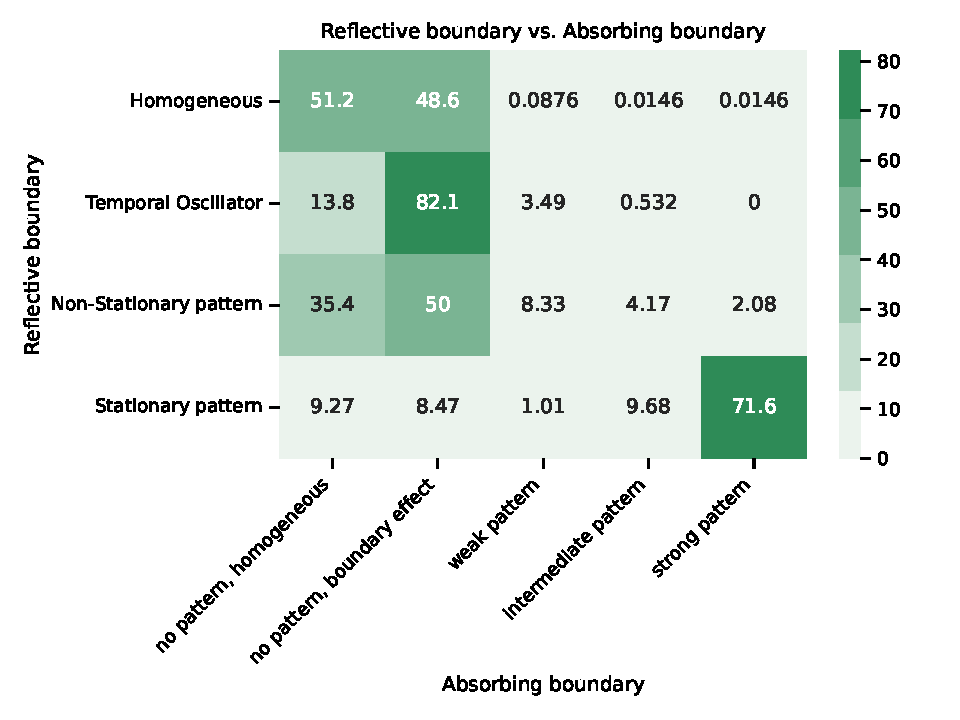
\includegraphics[width=1\textwidth]{chapters/Chapter 1/nogrowth_openboundary_confusion_variant0-11-12} % The name of your image file; assumes it is in the same directory as your .tex file
    \end{adjustbox}
    \caption{\textbf{Confusion matrix linking system outcome with reflective boundary and absorbing boundary.} Numbers show the percentage of solutions across the rows with reflective boundary output.}
    \caption{Effects of absorbing boundary conditions on patterning}
    \label{fig:nogrowth_openboundary_confusion_variant0} % A label for referencing this figure later in the document
\end{figure}

By studying the exceptions in this confusion matrix, we selected four interesting cases to display in this thesis, which helps us understand how absorbing boundary conditions might affect pattern formation.
Firstly, an homogenous oscillator under reflective boundaries might become a travelling wave when an absorbing boundary condition is introduced (Fig.~\ref{fig:interesting_cases_openboundary}A).
Absorbing boundary conditions can also help speed up the dynamics of pattern formation as seen in Fig.~\ref{fig:interesting_cases_openboundary}B where the pattern arises 20-fold faster than with reflective boundaries.
These types of boundaries can also help increase the dynamic range of the pattern as seen in Fig.~\ref{fig:interesting_cases_openboundary}C.
However, this might be the same effect seen in Fig.~\ref{fig:interesting_cases_openboundary}B where the reflective boundaries forming a pattern with longer time scales, therefore having a small dynamic range in earlier time points.
Finally, absorbing boundaries might also disrupt the pattern formation by reducing the pattern wavelength, as seen in Fig.~\ref{fig:interesting_cases_openboundary}D.
These results only correspond to a specific set of equations under a specific parameter distribution sampling.
However, other effects might occur when using other systems including model parameters and numerical parameters.

\begin{figure}[H] % h! is a placement specifier; it tries to place the image here.
    \centering
    \begin{adjustbox}{center}
        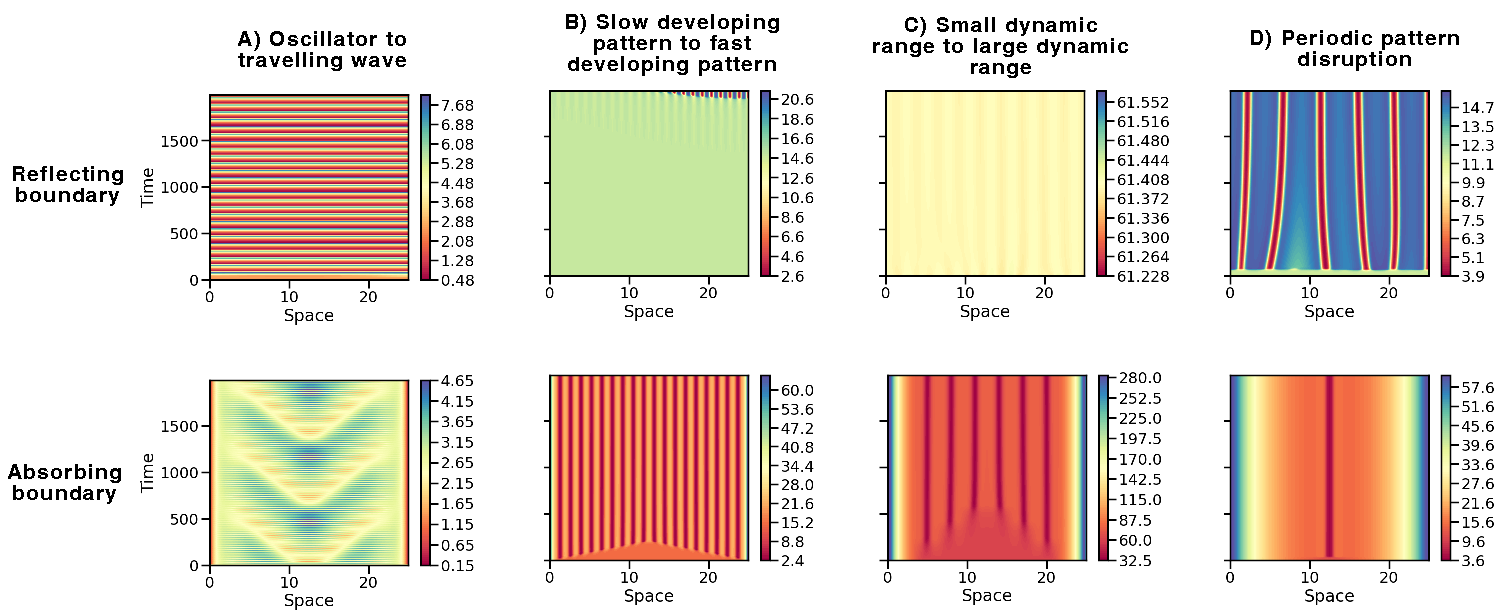
\includegraphics[width=1\textwidth]{chapters/Chapter 1/interesting_cases_openboundary} % The name of your image file; assumes it is in the same directory as your .tex file
    \end{adjustbox}
    \caption{\textbf{Examples of pattern transitions from reflecting boundaries to absorbing boundaries}. The system is simulated numerically in a non-growing domain using reflecting boundaries (top) and absorbing boundaries (bottom). Time-series numerical solution of A are shown for each case.}
    \label{fig:interesting_cases_openboundary}
\end{figure}

\subsection{Open boundaries to growth}
The patterning of the system is also studied when growth is added.
In this case, both non-growing and growing domains have absorbing boundary conditions so we can pinpoint the effects of growth.
The confusion matrix in Fig.~\ref{fig:openboundary_edgegrowth2_confusion_variant0} shows the correlation between non-growing and growing systems for 9,087 parameter sets.
Overall, we can see a strong diagonal, more populated in the bottom of the diagonal.
This suggests that growth often does not affect pattern formation, and when it does its more likely to destroy patterning.
Again, this result might be affected by the system of equations and the parameters used such as model parameters or numerical parameters (e.g.~length of the system or growth rate). %TODO discussion different growth rates might lead to increase or decrease robustness and to inner and outer growth formation.

\begin{figure}[H] % h! is a placement specifier; it tries to place the image here.
    \centering
    \begin{adjustbox}{center}
        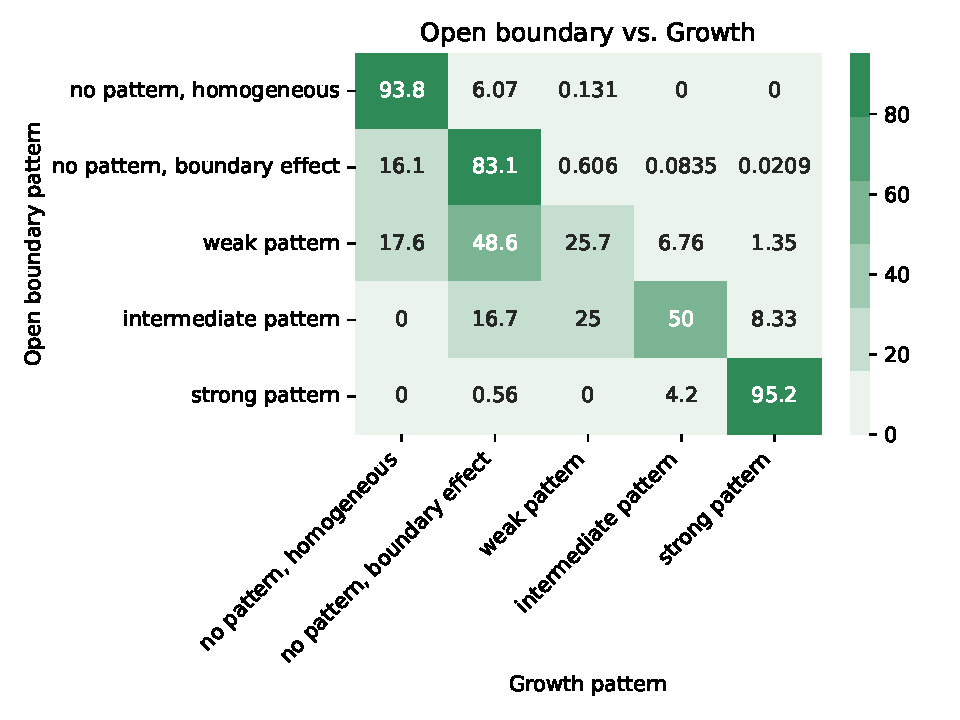
\includegraphics[width=1\textwidth]{chapters/Chapter 1/openboundary_edgegrowth2_confusion_variant0-11-12} % The name of your image file; assumes it is in the same directory as your .tex file
    \end{adjustbox}
    \caption{\textbf{Confusion matrix linking system outcome with no growth and linear growth.} Numbers show the percentage of solutions across the rows no growth. A strong diagonal of dark green squares is depicted, with which shows little effect when adding growth.}
    \label{fig:openboundary_edgegrowth2_confusion_variant0} % A label for referencing this figure later in the document
\end{figure}


From the confusion matrix, we investigated further some of the non-diagonal examples where growth added robustness, which are shown in Fig.~\ref{fig:interesting_cases_edgegrowth2}.
 However, in this case, the classification did not give good results.
This is mainly because non-stationary patterns could be classified into different categories depending on the time-point chosen, as the number of peaks varied over time.
Therefore, the comparison between growing and non-growing did not work as it ended up being a comparison between two time-points.(Fig.~\ref{fig:interesting_cases_edgegrowth2}A-B).
In some cases, we could identify patterns where the number of peaks increased just by having growth (Fig.~\ref{fig:interesting_cases_edgegrowth2}C).
Finally, we observe that in growing domains, we generally observe outer ring addition in for this system and growth rates (Fig.~\ref{fig:growing_pattern}).
\begin{figure}[H] % h! is a placement specifier; it tries to place the image here.

    \centering
    \begin{adjustbox}{center}
        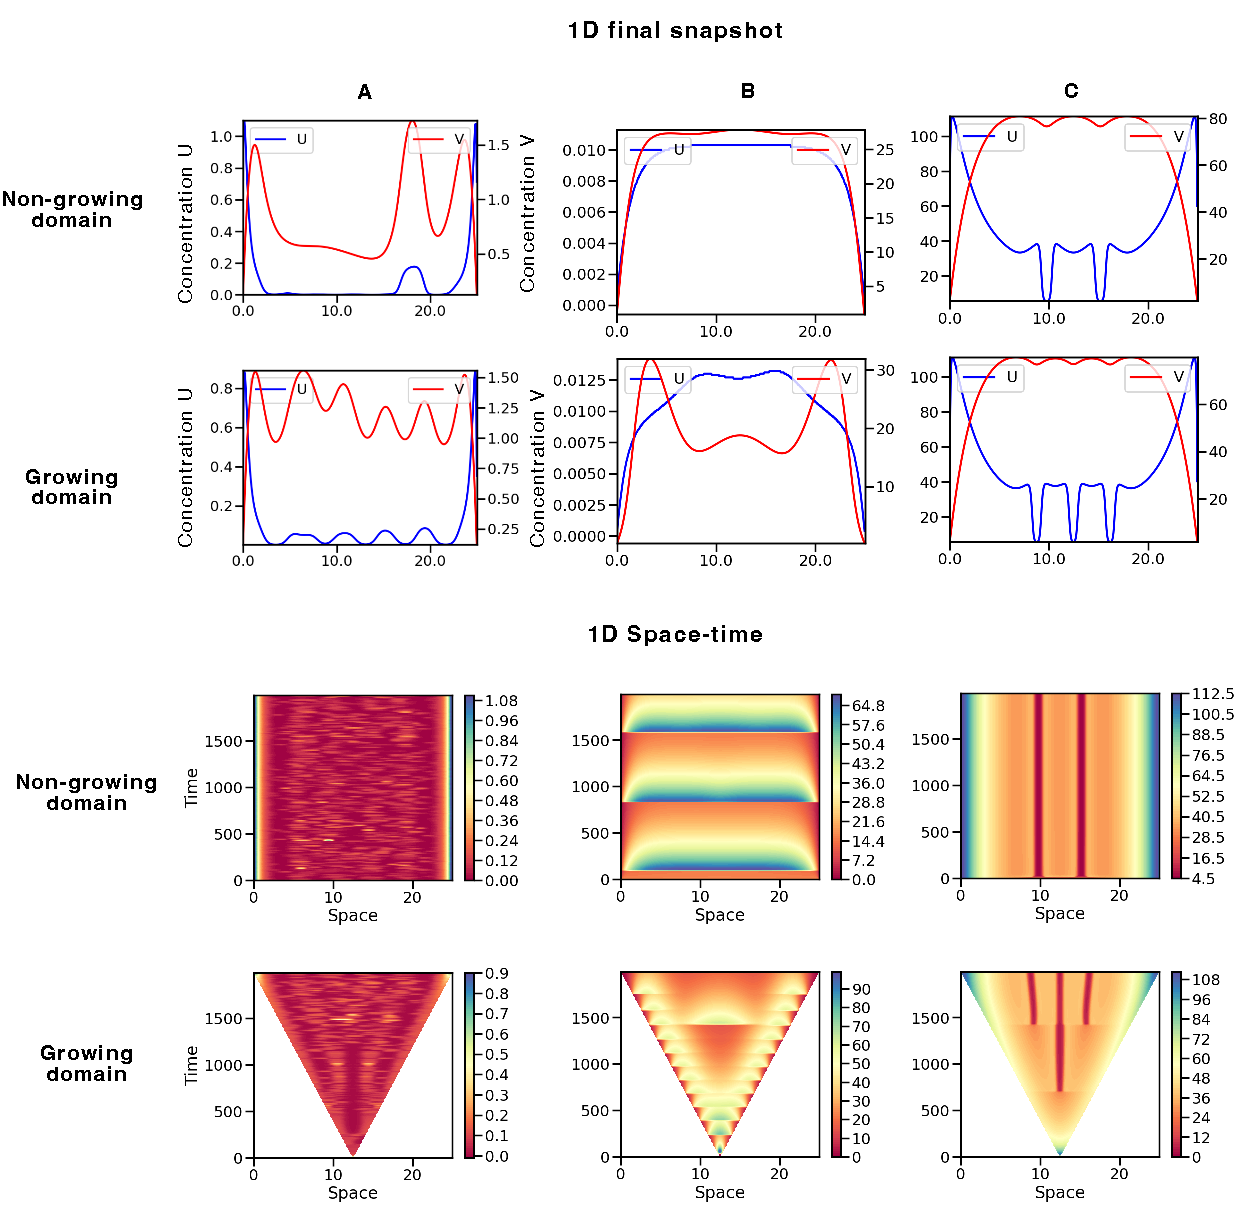
\includegraphics[width=1\textwidth]{chapters/Chapter 1/interesting_cases_edgegrowth2} % The name of your image file; assumes it is in the same directory as your .tex file
    \end{adjustbox}
    \caption{\textbf{Examples of pattern transitions from non-growing domains to linearly growing domains}. Three cases are shown. For each case we show both growing and non growing solutions, as well as final snapshot (i) and time-series (ii). Simulations were carried out with CN solver.}
    \label{fig:interesting_cases_edgegrowth2}
\end{figure}
%TODO remove top and bottom?
Finally, in Fig.~\ref{fig:3layer_sankey}, we can see a Sankey diagram which represents the flows from one type of pattern to another as absorbing boundaries and growth are added.
Pattern classes are ranked top-to-bottom from less patterned to more.
Overall, we can see a flow upwards towards less patterned outcomes as these effects are introduced.
However some flows go downwards, meaning absorbing boundaries and growth might convey robustness in some cases.

\begin{figure}[H] % h! is a placement specifier; it tries to place the image here.
    \centering
    \begin{adjustbox}{center}
        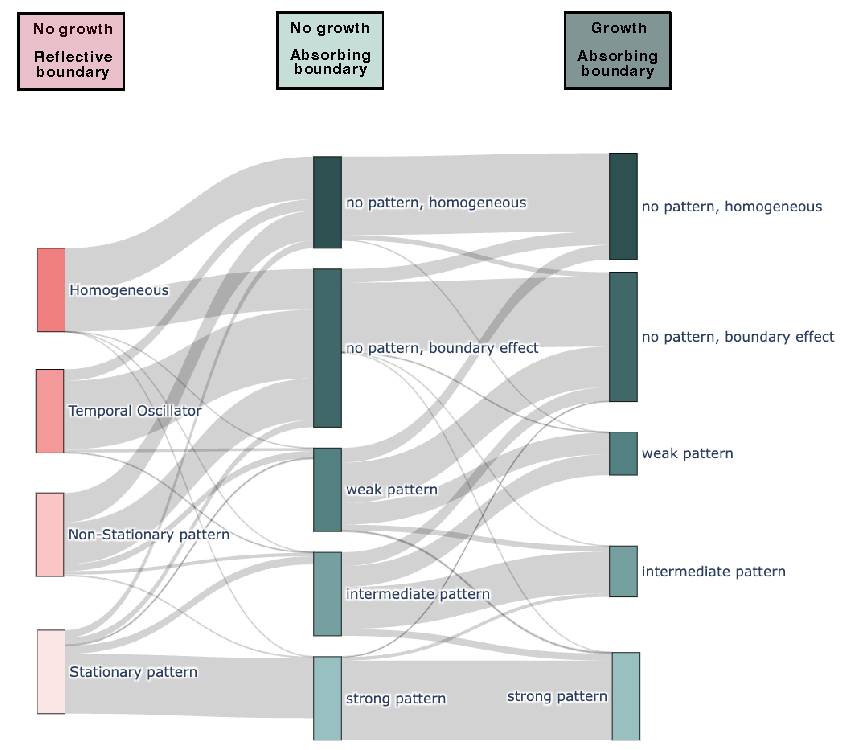
\includegraphics[width=1\textwidth]{chapters/Chapter 1/3layer_sankey} % The name of your image file; assumes it is in the same directory as your .tex file
    \end{adjustbox}
    \caption{\textbf{Sankey Diagram showing flow of pattern outcomes}. The 3 layer sankey shows the flows of patterns when going from reflective boundary conditions (left) to absorbing boundary conditions (center) to growth. Two color codes, pinks and blues, are used for the two types of classifications (Homogeneity-convergence decision tree and number of peaks)}
    \label{fig:3layer_sankey} % A label for referencing this figure later in the document
\end{figure}


\section{Discussion}
This chapter reflects all the fundamental work needed prior to investigating Turing patterns in the experimentally built genetic circuit.
Theoretical insights were obtained, that will later be applied in the following chapters.
For this reason, the basic Turing activator-inhibitor two node topology was chosen, which is easier to interpret and faster to compute results.
However, for results to be translatable to the experimental gene circuits, non-linear Hill terms were used to describe real genetic interactions between the two nodes.

\subsection*{Information in the dispersion relation}
We first started by understanding what information we could obtain by LSA about the patterns formed.
Current state of the art merely uses the dispersion relation to see if there is a diffusion-driven instability or not.
We went beyond this to derive relationships between the dispersion relation and the numerical wavelength, convergence time and pattern shape.
In the wavelength case, it seems like numerical patterns have a slightly bigger wavelength than the predicted wavelength from dispersion relation.
Unexpectedly, this relationship is not $y=x$, but $y=1.46x$.
Non-linearities might drive the system to choose lower slighly lower wavenumber modes which yield higher wavelengths numerically.
However a linear correlation holds, meaning we can still use LSA to predict pattern wavelength.
More cases with higher wavelengths would need to be investigated to understand if this correlation is generally maintained.

A negative correlation between dispersion height and convergence time to stationary patterns was found.
This can be explained, as a high eigenvalue leads to a faster exponential increase of the amplitude of the perturbations as seen in Eqs~\ref{eq: exponential form RD}, and therefore faster time-scales.
However, this correlation was less clear than in the wavelength study and only works well when studying related neighbouring patterns where a decaying exponential function is seen (Fig~\ref{fig:dispersion_peak_optimisation}B).
In non-neighbouring patterns (Fig~\ref{fig:dispersion_to_wavelength_convergence}B), this relationship did not capture the behaviour of patterns with low eigenvalues or low convergence time.
Overall, higher dispersion peaks point towards faster forming patterns, but this should be double checked with numerics if comparing patterns from different regions of the parameter space.

Finally, dispersion peak height also seemed to be an indicator of pattern shape in neighbouring regions of the parameter space.
Higher dispersion peaks led to spot-like patterns, while lower dispersion peaks led to labyrinthian patterns.
A potential explanation of this is that numerical patterns with lower dispersion peaks have not fully converged as their time-scales are slower, although patterns seemed to have qualitatively converged when the time-series were observed.
Future work should involve testing those simulations for larger times to ensure the hypothesis is correct.


\subsection*{Breaking linear stability analysis predictions}
Experimental work to engineer Turing patterns could benefit from faster-forming patterns as this would result in less stressed cellular tissues by avoiding nutrient depletion, accumulation of toxic molecules or cell death.
By looking at which parameters changed during the optimisation, we could tune the experimental circuit to modify those parameters and therefore tune our pattern time-scales.
Additionally, tuning pattern shape or wavelength could turn useful if different biotechnology applications require different morphologies or scales.
Although we have only shown optimisation for the case of dispersion peak height, the same optimisation could be carried out to choose a particular pattern wavelength.

As seen above, LSA can produce information on whether a system produces periodic stationary patterns and about the features of these patterns.
However, we have shown as well that these predictions are not as reliable as we might think, and numerical methods are therefore needed.
In this chapter we focused on how multistability might break these predictions, and how systems with other types of dispersion relations profiles can generate other stationary and non-stationary patterns.

Current literature does not explore multistability in Turing in detail.
High-throughput studies either do not mention multistability, or mention it but do not address it by discarding such cases ~\parencite{Scholes2019, Marcon, Zheng2016}.
Here we explored different cases of multistability and displayed the different potential outcomes of how the various states interact.
We showed the mechanism of how unstable systems can gain Turing pattern dynamics through multistability, as well as Turing states lose their patterning.
Additionally, we documented ephemeral patterns which are transient patterns occurring through as the system jumps from Turing to stable states.
These ephemeral patterns could still be interesting for developmental biology as the pattern can serve to temporarily activate the necessary genes to produce a non-transient phenotype (e.g. digit formation only needs periodic pattern at a specific time when the growth hormone is being produced to generate fingers~\parencite{Raspopovic1}.
Understanding how the interaction between different steady states affects pattern formation is key as multistability is extremely present and plays an important role in biological systems~\parencite{laurent1999multistability}.

In addition to multistability, current robustness studies do not explore alternative dispersion relations.
Here we showed how certain systems with unstable or Turing I-Hopf dispersion relations can generate Turing-like stationary periodic patterns (Fig.~\ref{fig:interesting_cases_nogrowth}).
Even though the robustness of these systems for periodic pattern formation is limited (Fig.~\ref{fig:lsa_numerical_confusion}), in certain regions of the parameter space Hopf and unstable systems robustly led to patterns in 100\% of the cases.
Therefore, systems with such dispersion relations should not be completely ruled out when studying pattern formation.
Considering them might increase the robustness slightly, however not enough to explain the difference between the robust mechanisms of nature and the non-robust Turing patterns.
Additionally, some systems with a Hopf dispersion relation produced interesting non-stationary periodic patterns.
These non-stationary patterns could be of great interest in the field of developmental and synthetic biology as gene expression arrest could turn them into periodic stationary patterns.
Additionally, these non-stationary patterns could serve as a periodic pre-pattern for the initial symmetry breaking.
Overall, when considering symmetric breaking events and periodicity in developmental biology, we should think beyond classical Turing dispersion relations and consider Hopf, Turing Hopf and simple unstable systems that might also explain periodic patterning in biology.

\subsection*{Introducing realistic biological phenomena: Absorbing boundaries and growth}
Following this theoretical route, we studied the effects of absorbing boundaries and growth in spatio-temporal patterns.
The motivation behind this was our experimental setup which involves Turing gene circuits in growing bacterial biofilms with absorbing boundary conditions.
Many studies have focused on understanding how growth or boundaries might affect pattern formation as seen in Section~\ref{growth_intro}.
However, these studies are extremely theoretical and hard to derive any assumptions for our experimental system.
Additionally, they are often based on complex analytical methods, yielding results which are hard to interpret.
For this reason, we performed a high-throughput numerical study to understand the effects that the type of growth and boundaries of our system has on patterning.
Our bacterial colonies grow in a linearly manner ~\cite{Tica2023}, where growth occurs mainly at the edges.
For this reason we generated this type of linear edge growth.
In terms of boundaries, empty agar absorbs the diffusors at the edge so we introduced absorbing boundary conditions.
However, the numerical parameters (length, growth rate, time) were not specifically those of our system as they had to be fined tuned to attain convergence, display enough peaks, and be computationally feasible.
Future work should focus on matching the numerical parameters to be more similar to our experimental system.

Overall, adding absorbing boundary conditions improved patterning more than adding growth.
Boundaries could induce robustness by generating non-stationary regular patterns or increasing speed of pattern formation.
However, patterns could also be disrupted by adding absorbing boundaries (Fig.~\ref{fig:interesting_cases_openboundary}).
As previously mentioned, non-stationary regular patterns might be extremely interesting for developmental biology as well as biotechnology applications.
Additionally, increasing the speed of pattern formation could be favourable to detect the patterns within the time duration of the experiment.

On the other hand, the growth used did not seem to improve robustness for pattern formation as more cases ended up in the bottom of the diagonal in the confusion matrix (Fig.~\ref{fig:openboundary_edgegrowth2_confusion_variant0}).
This goes against the literature which describes growth induced Turing patterns ~\parencite{gaffney2010}).
This might be because growth rates and types of growth (exponential or logistic) produce different results.
The growth rate used here was slower than the experimental growth rate as long times were initially simulated to reach convergence in the non-growing reflective boundaries case.
Future work should focus on testing robustness for the specific growth rates of our system.
Alternatively, insights into which growth rates promote pattern formation the most could be useful to tune experiments accordingly.

The main unresolved challenge of this chapter was optimising the classification methods to correctly classify patterns.
Firstly, two different classification methods were used which made comparing results harder.
Additionally, many patterns were misclassified, which meant the results were not necessarily statistically significant.
However, the method still allowed to find interesting cases where growth or boundaries affected patterning.
Better fine-tuning of threshold parameters or new classification methods are needed to avoid misclassification.
Fine-tuning the thresholds is an extremely difficult task due to the wide variety of solutions with different dynamic ranges, time-scales and wavelengths.
This can be solved by simulating larger fields, however this is computationally expensive.
Additionally, the peak number classification used for the solutions with absorbing boundary conditions and growing domains relied only on final snapshots.
This was mainly a problem when classifying non-stationary patterns as the number of peaks in these solutions increases and decreases over time, which might lead to misclassification.
A potential way forward could be to analyse image datasets with deep learning methods to classify resulting patterns without relying on manually set rules or thresholds.